\section{Introduction}

\subsection{The goal of this work}
The main topic of this work in the annihilation of composite antinuclei in nuclear matter. This process -- by which one or all of the antinucleons interact and annihilate with nucleons -- destroys the antinucleus in the process. Because of these annihilations, antinuclei are some of the rarest stable objects in our matter dominated\footnote{It remains of the biggest mysteries of physics why our universe is dominated by matter over antimatter, as the Big Bang should have produced them in equal amounts.} universe, as once produced they tend to annihilate quickly on cosmic timescales. And only very rare process even create antinuclei in the first place. \\
But this rarity is why antinuclei have received increased attention in recent years\cite{}, since any process which gives a signal by producing antinuclei does not have to contend with large backgrounds, but can be searched for with hope for a clean signal. In particular, theories which go beyond the current standard model of physics and can produce antinuclei, often hail them as a golden channel for detection. But in order to make any inference from future antinuclei measurements from such processes, their properties must be known, including the chance by which they might annihilate before reaching our detectors. One theory in particular has a vested interest in antinuclei: the weakly-interacting-massive-particle (WIMP) dark matter model. Some versions of this model predict dark matter annihilations into antinuclei, which could enable an indirect channel into unveiling the nature of dark matter.\\

So this effort to aid the search for new physics thus joins two separate fields of study: high-energy physics, which allows us to produce and study the properties of antinuclei on earth, and the search for signals of dark matter in cosmic rays, in particular antinuclei. The goal of this work is to present the work which was done during my PhD: the measurement of the inelastic cross sections of the $A$=3 antinuclei, and the effect of the measured antinuclei inelastic cross sections on an antinuclei signal in cosmic rays near earth. 

\subsection{The standard model of particle physics}
In this section a brief introduction to the standard model of particle physics is given, in order to introduce the terminology and concepts which will be used in this thesis. 
The standard model of particle physics describes the forces by which elementary particles interact with each other: the strong force, as described by quantum chromodynamics (QCD), the electromagnetic force as described by quantum electrodynamics (QED) and the weak force as described by electroweak theory (EWT). The standard model has been incredibly successful in describing the three forces. The forth fundamental force of nature, gravity, completes the description of nature, however, it remains unknown how to incorporate it into the standard model. Additionally, there are phenomena which are currently inexplicable within the standard model, notably dark matter and dark energy. This has prompted many searches for physics beyond the standard model (BSM), in order to complete our understanding of nature. So far however, these searches have remained without success. \\

In the standard model, there are 4 types of elementary particles: quarks, leptons, gauge bosons and the higgs scalar boson, which are summarized in figure \ref{fig:StandardModelParticles}. There are 3 generations of quarks and leptons, which differ from previous generations in their mass. Quarks are split into up-like quarks, with a $+\frac{2}{3}$ electric charge\footnote{Charges of elementary particles are given in multiples of the magnitude of the electron charge $e$.}, and down-like quarks with a $-\frac{1}{3}$ electric charge. Leptons are split between charged leptons with charge $q=-1$ and neutrinos, which carry no electric or color charge, and are very light. There are 4 gauge bosons for the 3 fundamental forces which the standard model describes: the gluon ($g$) for the strong force, the photon ($\gamma$) for the electromagnetic force, and the W and Z bosons for the weak force. The weak bosons couple to all quarks and leptons as well as themselves, while photons couple to electrically charged particles (quarks and charged leptons), and gluons couple to quarks, since they carry a color charge\footnote{Color charge is the QCD equivalent of the electric charge.}. Additionally, gluons can interact with themselves, since they also carry the color charge of the strong force.
Finally, there is the scalar higgs boson, which is responsible for the mechanism which gives particles their mass.
All quarks and leptons also have a corresponding antiparticle, with the same mass, spin and lifetime, but with all other quantum numbers inverted according to the charge, parity and time reversal (CPT) symmetry\footnote{Further information about CPT symmetry can be found in any university level physics textbook, such as \cite{}, and in section \ref{sec:IntroSymmetries}.}. \\

\begin{figure}[h!]
    \centering
    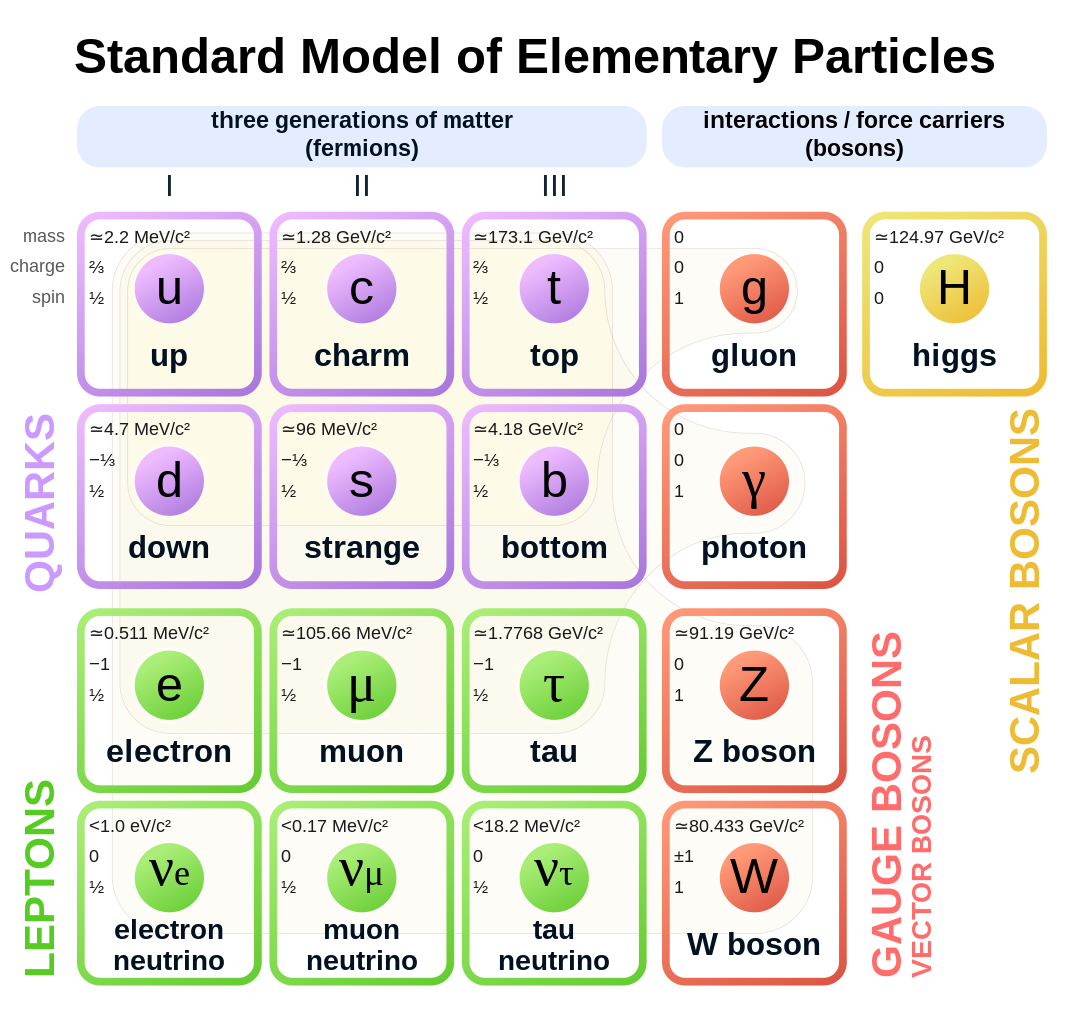
\includegraphics[width=0.7\textwidth]{figures/Standard_Model_of_Elementary_Particles.svg.png}
    \caption{The particles of the standard model of particle physics. There are 3 generations of quarks and leptons, which differ from previous generations only in their mass. Quarks are split into up-like quarks, with a $+\frac{2}{3}$ charge, and down-like quarks with a $1\frac{1}{3}$ charge. Leptons are split between charged leptons with charge $q=-1$ and neutrinos, which carry no electromagnetic or color charge, and are very light. There are 4 gauge bosons for the 3 fundametal forces which the standard model describes: the gluon ($g$) for the strong force, the photon ($\gamma$) for the electromagnetic force, and the W and Z bosons for the weak force. Additionally, there is the scalar higgs boson, which is responsible for the mechanism which gives other particles their mass.}
    \label{fig:StandardModelParticles}
\end{figure}


Quarks always form composite particles made up of either three quarks (baryons) or a quark-antiquark pair (mesons). %i know there are also pentaquarks, but they have nothing to do with this thesis and are therefore not mentioned
These two differ in the fact that baryons are fermions (half integer value spin) and mesons are bosons (integer value spin). The baryon number\footnote{The baryon number is a quantum number where baryons have 1 and antibaryons have -1.} is also conserved in all known reaction of the standard model, which means that the relative number of baryons-antibaryons remains constant. \\
It is important to note why quarks are never found individually. Quarks carry color charge, which is the charge of the strong force. The shape of the strong force does not allow for isolated color charges to exist, a principle called  color confinement. Unlike for example the electromagnetic force, which gets weaker as the distance between two particles grows, the strong force remains constant. The potential of the strong force can thus be phenomenologically described by the Cornell potential\cite{Strong_potential}, as given in equation \ref{eq:StrongPotential}:
\begin{equation}\label{eq:StrongPotential}
    V(r) = -\frac{4}{3}\frac{\alpha_s}{r}+\kappa r
\end{equation}
, where $\kappa$ is constant. The second term of equation \ref{eq:StrongPotential} dominates at large radii (>1 fm), and is thus responsible for the long distance behavior of the strong force. The energy stored in the field between two particles can be found by $\delta E(r_1-r_0) = V(r_1)-V(r_0) = \int_{r_0}^{r_1} \vec{F}.d\vec{r}$, i.e. the path integral of the force along the separation between the particles. If the force decreases enough\footnote{If the force decreases as 1/$r$, the integral of $\int_{x_0}^{\inf} \frac{1}{\vec{r} } .d\vec{r} \propto \mathrm{ln}(r)$ will go to infinity at infinite distances, therefore the force simply decreasing is not sufficient. However, if the force decreases as 1/$r^2$ -- as it does for the electromagnetic and gravitational forces -- the integral is finite at infinite distances.} as the distance grows, this allows potential energy to be stored in the field between two particles, without this energy becoming infinitely large at large distances. However, if the force remains constant even with larger distances, the energy stored in the field increases proportionally to the distance between particles. For the strong force, this gluon field between two particles which are being separated is often called a string. Eventually, enough energy is stored in the string that a new antiquark-quark pair can be created, isolating the color charges at each end of the string, thus splitting the string in two. The mount of energy stored in gluon strings is estimated to be roughly 1 GeV/fm\cite{}. This mechanism, which is shown in figure \ref{fig:IntroStringFragmentation}, is called string fragmentation, and is an intuitive explanation for why the color charges of the strong force cannot be isolated. \\

\begin{figure}[h!]
    \centering
    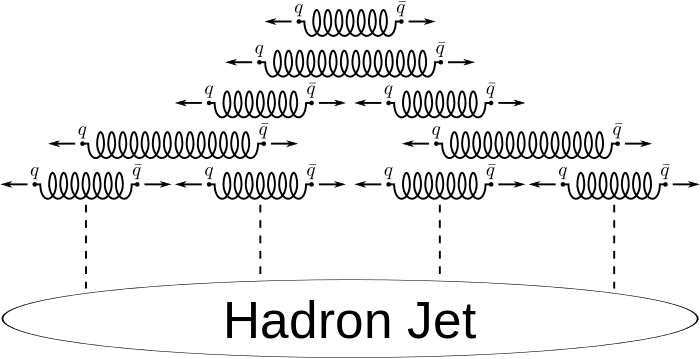
\includegraphics[width=\textwidth]{figures/String_fragmentation.png}
    \caption{Color confinement by string fragmentation. As the antiquark-quark pair moved away from each other, more and more energy is stored in the color flux tube between them. Eventually, there is sufficient energy to create a new quark-antiquark pair, and thus truncate the flux tube. This process continues until the (anti)quarks run out of sufficient energy to create new quark-antiquark pairs. The quarks can then hadronise. The figure is taken from \cite{StringFragmentationGraphic}.}
    \label{fig:IntroStringFragmentation}
\end{figure}




\subsubsection{Symmetries and symmetry breaking within the standard model}\label{sec:IntroSymmetries}
Symmetries are a fundamental aspect of the standard model. A symmetry can be defined as a global operation under which the laws of physics remain the same, and they can be deceptively powerful. In fact, something as fundamental as conservation of energy can be shown to be equivalent to a symmetry to translations in time. Other continuous symmetries such as spatial translation and spatial rotation give rise to conservation of momentum and angular momentum, respectively\footnote{The relations between physical symmetries and conservation laws was established by Noether's first theorem \cite{Noether1918}. }. But there are also symmetries which are not continuous, but discrete\footnote{In order to distinguish between a continous and discreet symmetry, consider the difference between spatial translations and spatial inversions. The first is an operation which moves a system to a different point in space. It does not matter if the movement happens by 1m or 1km, the symmetry should hold all the same and is thus considered continous. Meanwhile, spatial inversion inverts the direction of the axes, similar to how a mirror inverts one axis. This is not a continuous operation, since it is impossible to "half-mirror" an object.}. The standard model of particle physics contains three important and related discrete symmetries\cite{}. Under these symmetries, the laws of physics are expected to behave the same. C-symmetry, which stands for charge and represents replacing particles with their antiparticles. P-symmetry, which stands for parity symmetry, which represents spatial inversion along the 3 physical axes. And finally T-symmetry, which stands for time-inversion symmetry, which represents inversion of the direction of time. \\

They are called near symmetries, because each of them is individually broken within the standard model. A symmetry can be broken in two ways: explicitly or spontaneously. Explicit symmetry breaking is when the Lagrangian corresponding to an interaction does not itself respect the symmetry, while spontaneous symmetry breaking is when the Lagrangian respects the symmetry, but its ground state solution does not. The most famous individual violation is the breaking of P-symmetry of the weak force, which couples only to left-handed fermions and right-handed antifermions. In other words, a system of fermions and antifermions inverted under P-symmetry would no longer couple to the weak force, as the fermions are now right handed and the antifermions left handed. It is then obvious that replacing particles by their antiparticles would restore this symmetry. This combined symmetry is called CP-symmetry, and is thought to be respected by the strong and electromagnetic forces, however, there is a degree of CP violation in the mixing of different quark generations by means of the weak force, as described by the Cabbibo-Kobayashi-Masakawa (CKM) matrix. Introducing a complex phase in the quark mixing allows for the weak force to violate CP symmetry\cite{}. 

This can be exemplified by the following consideration. Consider a process $a \rightarrow b$, and the corresponding process with the antiparticles $\bar{a} \rightarrow \bar{b}$ and denote the amplitudes with $M$ and $\bar{M}$. By CP symmetry (i.e. before the violation), these numbers must be the same. We can separate them into a magnitude and a phase as $M = \bar{M} = |M|e^{i\theta}$. If there is a complex phase term introduced (for example by the CKM matrix) the amplitudes become $M = |M|e^{i\theta}e^{i\phi}$ and $\bar{M} = |M|e^{i\theta}e^{-i\phi}$. Since measurable rates are proportional to $|M|^2$, CP symmetry is still conserved. However, now consider the case where the reaction can take two different routes, $a \rightarrow 1 \rightarrow b$ and $a \rightarrow 2 \rightarrow b$ and the amplitudes become: $M = |M_1|e^{i\theta_1}e^{i\phi_1} + |M_2|e^{i\theta_2}e^{i\phi_2}$ and $\bar{M} = |M_1|e^{i\theta_1}e^{-i\phi_1} + |M_2|e^{i\theta_2}e^{-i\phi_2}$. This allows the calculation of the differences in amplitudes as $|M|^2 - |\bar{M}|^2 = -4|M_1||M_2|\mathrm{sin}(\theta_1 - \theta_2)\mathrm{cos}(\phi_1 - \phi_2)$. Thus, the introduction of a complex phase causes a violation between matter and antimatter. \\
CP violation was first observed in the decays of neutral Kaons\cite{CP_violations_early} in 1964, and was confirmed in 1999 \cite{CP_violations_proof}. Since then it has also been observed in the decays of $B$ and $D$ mesons \cite{CP_violation_B, CP_violation_D}. CP violation is also necessary (but not sufficient) in order to produce the matter-antimatter asymmetry, as is elaborated in section \ref{sec:IntroSakharovContidion}. Even though the CP symmetry is being violated, the combined CPT symmetry is expected to be conserved in all standard model processes\cite{}. 

Lastly, let us consider what is known as the strong CP problem. The QCD Lagrangian must include a CP violating term in order to account for the difference between the pion and $\eta$ masses \cite{tHooft}, which is characterised by a free parameter $0<\bar{\theta}<2\pi$. But by measurements of the neutron electric dipole moment it has been shown that $\bar{\theta} \lesssim 10^{-10}$. This represents a fine tuning problem: there must be a CP violating term in QCD, but it must also be set to be almost 0. So far, only one convincing solution has been introduced: the Peccei-Quinn (PQ) model. This model introduces a new global symmetry to the QCD Lagrangian, and a corresponding scalar field. This symmetry is then spontaneously broken at low energies, creating the axion\footnote{The name axion comes from a brand of laundry detergent, and was chosen because the axion "cleans up" the strong CP problem.}, a promising alternative dark matter model. For a more detailed mathematical description of the axion see \cite{axion_review}.


\subsection{Matter and antimatter in the universe}


\subsubsection{Origin of baryonic matter}
The majority of the baryonic matter we see in the universe was created within the first instances after the Big Bang. Initially, the universe was in a hot dense state, with temperatures much higher than the masses of the elementary particles. In fact, the temperature was so high that the higgs mechanism did not yet provide mass to particles\cite{Higgs_vev_highT} (T $\gtrsim 150$ GeV). During this time, quarks, leptons and bosons were in a thermodynamic equilibrium. As the universe underwent inflation, it became colder and colder, until eventually the higgs mechanism started to make particles massive\cite{Higgs_vev_highT} (see section \ref{sec:IntroBaryogenesisSM} for more details). This phase transition of the universe is one option for the source of the matter excess in the universe.
As the universe continued to evolve and temperatures cooled, quarks and gluons first formed a quark-gluon plasma -- a state of matter in which color charges can move freely\cite{} --  and eventually hadrons, which decay leaving only the most stable hadrons (protons and neutrons) behind. At this point about 1s had passed since the Big Bang. From about 10s to 20 minutes after the Big Bang, the temperatures enabled nuclear fusion. It was during this time that most of the deuterium, helium-4 and lithium in the universe were formed. \\

\begin{figure}
    \centering
    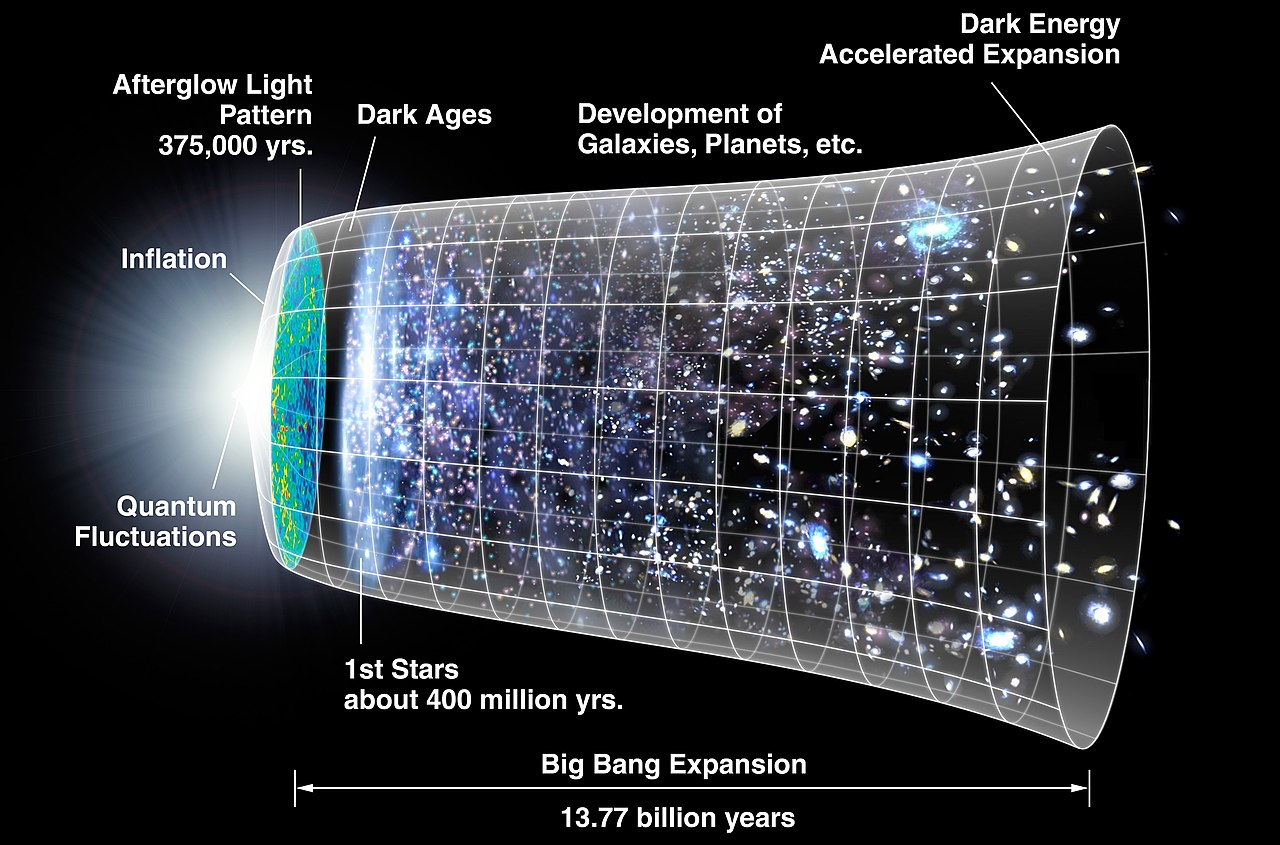
\includegraphics[width=\textwidth]{figures/CMB_Timeline300_no_WMAP.jpg}
    \caption{Timeline of the universe, starting from the Big Bang \cite{timelineOfTheUniverse}.}
    \label{fig:TimelineOfTheUniverse}
\end{figure}

The immediate period after the big bang shaped our universe in more ways than simply creating an excess of matter over antimatter. The gravitational collapse of dark matter during this time is thought to be responsible for the formation of galactic structures\cite{Ibarra_neutrinos}. The creation of nuclear matter determines the majority of the make up of the universe to this day. The timeline of the evolution of the universe is shown in figure \ref{fig:TimelineOfTheUniverse}.

\subsubsection{A matter dominated universe: antimatter-matter asymmetry}
To the best of our knowledge our universe is  entirely dominated by matter over antimatter. This observation is staggering, because in all the reactions we can observe in particle physics experiments near earth, whenever new matter is produced the same amount of antimatter is produced as well. So the a priori assumption is that the universe houses as much antimatter as it does matter. And at first glance, this doesn't seem to impose any impossible constraints, as from a distance matter and antimatter are indistinguishable\footnote{This means to say that matter atoms would produce the same spectral lines as antimatter atoms, and undergo the same fusion reactions we see in stars.}. So while our solar system might be made of matter, what is to keep other solar systems, or even other galaxies from being made of antimatter? The issue arises when we look at the surroundings of solar systems or galaxies. Interstellar/intergalactic space is not completely empty, but populated at very low densities by protons and helium-4 from surrounding stars/galaxies. We know the density of protons in these regions to be about $n_\mathrm{H} \approx 1$ cm$^{-3}$ for interstellar space\cite{}, and $n_\mathrm{H} \approx 1$ m$^{-3}$ for intergalactic space \cite{}. And when a matter dominated region and an antimatter dominated region are next to each other, then in this vast space of low density matter, plenty of annihilations would occur. These annihilations would produce distinctive signals in gamma ray searches, due to high energy photons emitted from $e^+e^-$ annihilations or from the decay of $\pi^0$s produced in $\mathrm{p}\overline{\mathrm{p}}$ annihilations\cite{Schönfelder1989}. The lack of any such signals places stringent limits on any large areas of antimatter within the observable universe, and leads us to believe that our universe is indeed dominated by matter. The source of this matter-antimatter asymmetry is one of the big remaining mysteries of physics.  \\

It isn't known exactly how the different populations of matter and antimatter came to be. Perhaps only a minute difference between the two caused a tiny fraction more matter to be produced than antimatter. And since the majority of both annihilated, what we see today might by this tiny leftover fraction. For this reason, searches for differences between matter particles and their antimatter counterparts are looking to find even the tiniest discrepancy between the two\cite{}. 

\subsubsection{Sakharov condition}\label{sec:IntroSakharovContidion}
Given the a priori assumption that the same amount of matter and antimatter would be produced, it is necessary to clarify the conditions under which this could be altered. In \cite{Sakharov:1967dj}, the necessary conditions for the creation of a baryon excess were shown to be:
\begin{itemize}
    \item Some interactions of elementary particles must violate baryon number conservation, since the net baryon number of the universe must change over time
    \item C and CP must be violated so that there is no equality in the forward and backward rates of the baryon number violating processes. 
    \item The net flux must be created in out-of-equilibrium conditions, since otherwise CPT symmetry would assure compensation of the effect. 
\end{itemize}

The first condition is trivial. The second condition means that there must be a reaction which differentiates between the matter and antimatter, in order to give rise to a process which would preferably create baryons over antibaryons. The third condition requires some more explanation. It is based on the fact that we believe the CPT symmetry to be exact. Therefore, there must be a process which only happens in one direction in time. This cannot occur in an equilibrium condition, since in equilibrium all reactions occur in both the forward and backward directions. Therefore, it must be a reaction linked to out-of-equilibrium processes. 


\subsubsection{Baryogenesis within the standard model}\label{sec:IntroBaryogenesisSM}
It is possible to account for the matter-antimatter asymmetry in the universe through standard model processes. One such process was outlined in \cite{Bubbles_asymmetry}. The main arguments of this paper are reproduced here, to exemplify how the Sakharov condition above can be applied. \\

The main idea of the mechanism is threefold: i) the existence of a first order phase transition as the universe cools below the electroweak phase transition. The phase transition satisfies the out-of-equilibrium part of the Sakharov conditions. ii) quarks and antiquarks scattering of the phase boundary in an asymmetric fashion, due to CP-violating effects. This results in a net baryon flux through the phase boundary. And iii), the excess antiquarks in the hot medium are removed by an effect which does not conserve baryon number, before the phase transition is complete in the entire universe. \\
In the standard model, particles get their mass by their Yukawa coupling to the higgs vacuum expectation value\cite{SANTAMARIA199390}. The vacuum expectation value of the higgs field vanishes at temperatures above the electroweak phase transition, such as were present during the early universe\cite{Higgs_vev_highT}. If this phase transition is treated as a first order phase transition, with bubbles of the colder phase forming out of the hot medium, then the vacuum expectation value of the higgs will change while crossing the phase boundary. This will change the masses of fermions as they move across this phase boundary, which thus acts as a potential barrier. This causes both quarks and antiquarks to scatter from this barrier. However, due to the CP-violating nature of the weak interaction, the transmission through the barrier can be different for quarks and antiquarks, resulting in a baryon flux through the phase boundary. Excess antiquarks in the medium are then removed by sphalerons. A sphaleron is a solution to the electroweak field equations, geometrically represented by a saddle point which connects a 3 baryon system to a 3 antilepton system\footnote{And equivalently 3 antibaryons to 3 leptons.}\cite{Phong_2020}. Sphaleron effects are expected to be frozen out below about 10 TeV. Since the temperature is higher on one side of the phase transition than the other, the baryon number symmetry violating process is hypothesised to occur only on the hot side, and thus leave a net baryon number.  \\

While sphalerons are currently hypothetical, it is expected that the high luminosity upgrade of the LHC will be able to start the experimental search for sphalerons \cite{Papaefstathiou_2019}.


\subsection{Antimatter-matter annihilations}
The lightest quarks -- $u$ and $d$ -- make up normal nuclear matter, i.e. protons $uud$ and neutrons $udd$, which are the two lightest baryons with masses of 938 MeV/$c^2$ and 939 MeV/$c^2$, respectively. Since the proton is the lightest baryon, and the baryon number must be conserved, any reaction of the proton with other matter must leave an intact proton at the end, thus never making the energy stored in the proton's mass available to create new particles. When baryons interact with their antibaryons, they annihilate, releasing their entire mass as available energy to create new particles. This is because by definition, the total baryon number of such a reaction is 0. The same is true for the annihilations of leptons and lepton number conservation, and for the conservation of electric charge in the annihilations of leptons and baryons. In principle, if a quantum number is antisymmetric under the C symmetry, it will be conserved by construction in antimatter-matter annihilation events and thus will never limit the available phase space of reactions. \\

\subsubsection{Annihilation of $q\bar{q}$ and $l\bar{l}$ pairs}

It is simplest to start with the Feynman diagrams for the annihilations of elementary quarks and leptons. The lowest order diagrams are given in figure \ref{fig:annihilationsFeynmanElementary}. Their relative contribution is proportional to the force's interaction strength to the exponent of the number of vertices, so $\alpha$ for the electromagnetic force, $\alpha_w$ for the weak force and $\alpha_s$ for the strong force. At low energies, the three parameters have an ordering $\alpha_s$>>$\alpha$>>$\alpha_w$\footnote{The couplings depend on the energy scale, as all of them are running coupling constants. At high energies, the weak force is actually stronger than the electromagnetic force. This difference is due to the mass of the weak bosons.}. Essentially, quark and leptons can annihilate with their antiparticles through electromagnetic and weak channels, which can also convert from quarks to leptons and vice versa. Quarks can additionally annihilate via a gluon into either another quark-antiquark pair or into hadron jets. For quarks, annihilation through the strong force should outweigh annihilation through the electromagnetic force by a factor $\alpha_s^2/\alpha^2 >>1$, which means that the strong channel should dominate. 

\begin{figure}
    \centering
    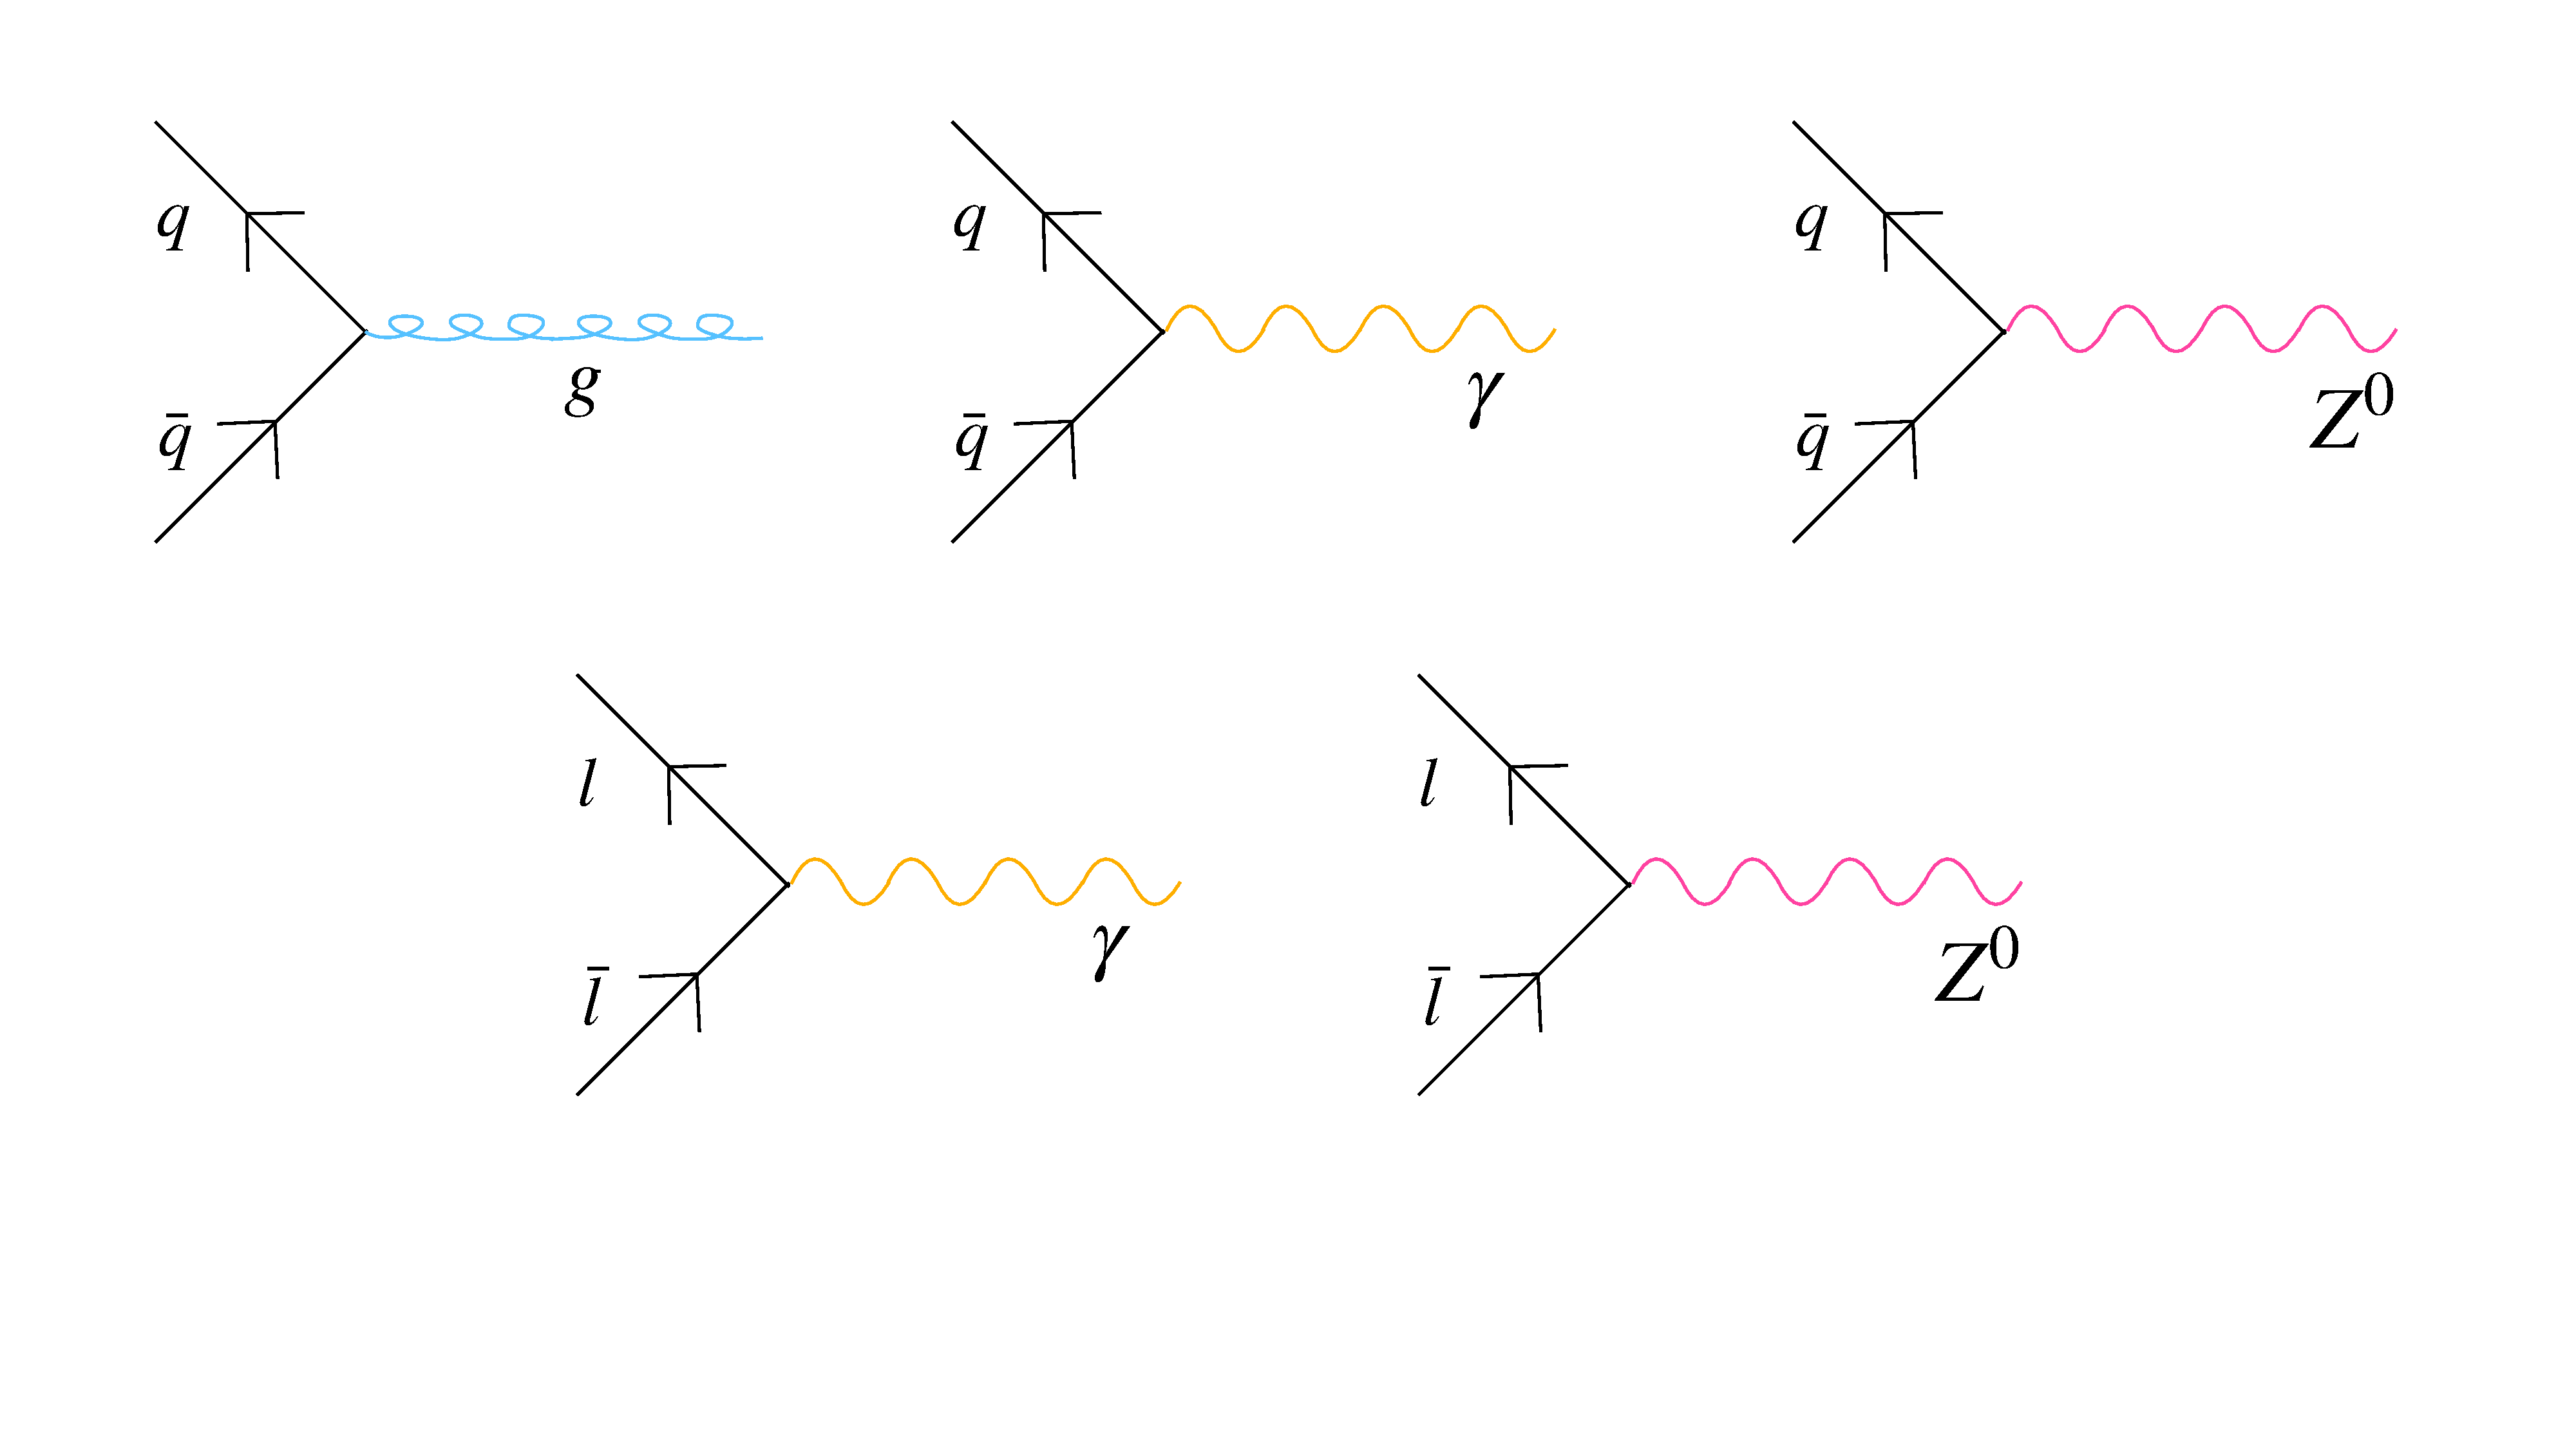
\includegraphics[width=0.9\textwidth]{figures/Annihilation_Feynman_diagram.pdf}
    \caption{First order Feynman diagrams showing the annihilations of elementary particles. Top row: quark-antiquark annihilation through the strong (left), electromagnetic (middle) and weak (right) force. Bottom row: lepton-antilepton annihilation through the electromagnetic (left) and weak (right) force.}
    \label{fig:annihilationsFeynmanElementary}
\end{figure}

\subsubsection{Antiproton-proton annihilations}
It is important to note at the start of this chapter that there is currently no theory or even model which can describe the available data for antiproton-proton annihilations, or offer up an explanation for the underlying mechanism\cite{antiproton_cross_sections_review}. This is in stark contrast to quark-antiquark annihilation, which is just a first order QCD process. In this section I shall attempt to give an overview of the difficulties in describing this process, and thereby offer up a qualitative picture of the possible annihilation mechanisms.\\

It is tempting to assume that in order to scale up an annihilation event, one might just be able to scale up the single Feynman diagrams for quark-antiquark annihilation in order to get a description for antiproton-proton annihilation. However, the picture is far more complicated. This can be intuitively understood by the fact that (anti)protons are made up of 3 valence (anti)quarks, but in the annihilation of (anti)proton pair, some of their valence (anti)quarks may well survive. In fact, consider the following reaction $\matrm{p\bar{p}} \rightarrow 3 \mathrm{M}$, where M denotes a meson. This reaction can occur by simply rearranging the quark content of the proton and antiproton, which is illustrated in figure \ref{fig:Quark_Rearrangement}. Such a rearranging of the quarks can happen if the quarks can feel each others strong potential, which can be mediated through pion exchange. This can be seen as equivalent to nucleon-nucleon interactions through pion exchange, at distances beyond the confines of color confinement. This effectively allows the potential for quark rearranging to be felt at further distances than the potential for quark-antiquark annihilation. The annihilation potential between an antiproton-proton pair therefore can have a long range ( $\gtrsim 1$ fm ) and a short range ($\lesssim 1$ fm) term, where the long range term is dominated by the rearrangement of quarks and antiquarks into mesons, and the short range term is dominated by quark-antiquark annihilation. The common notation of these processes is $An$ and $Rn$ for annihilation ($A$) and rearrangement ($R$) into $n$ mesons.\\

\begin{figure}[h!]
    \centering
    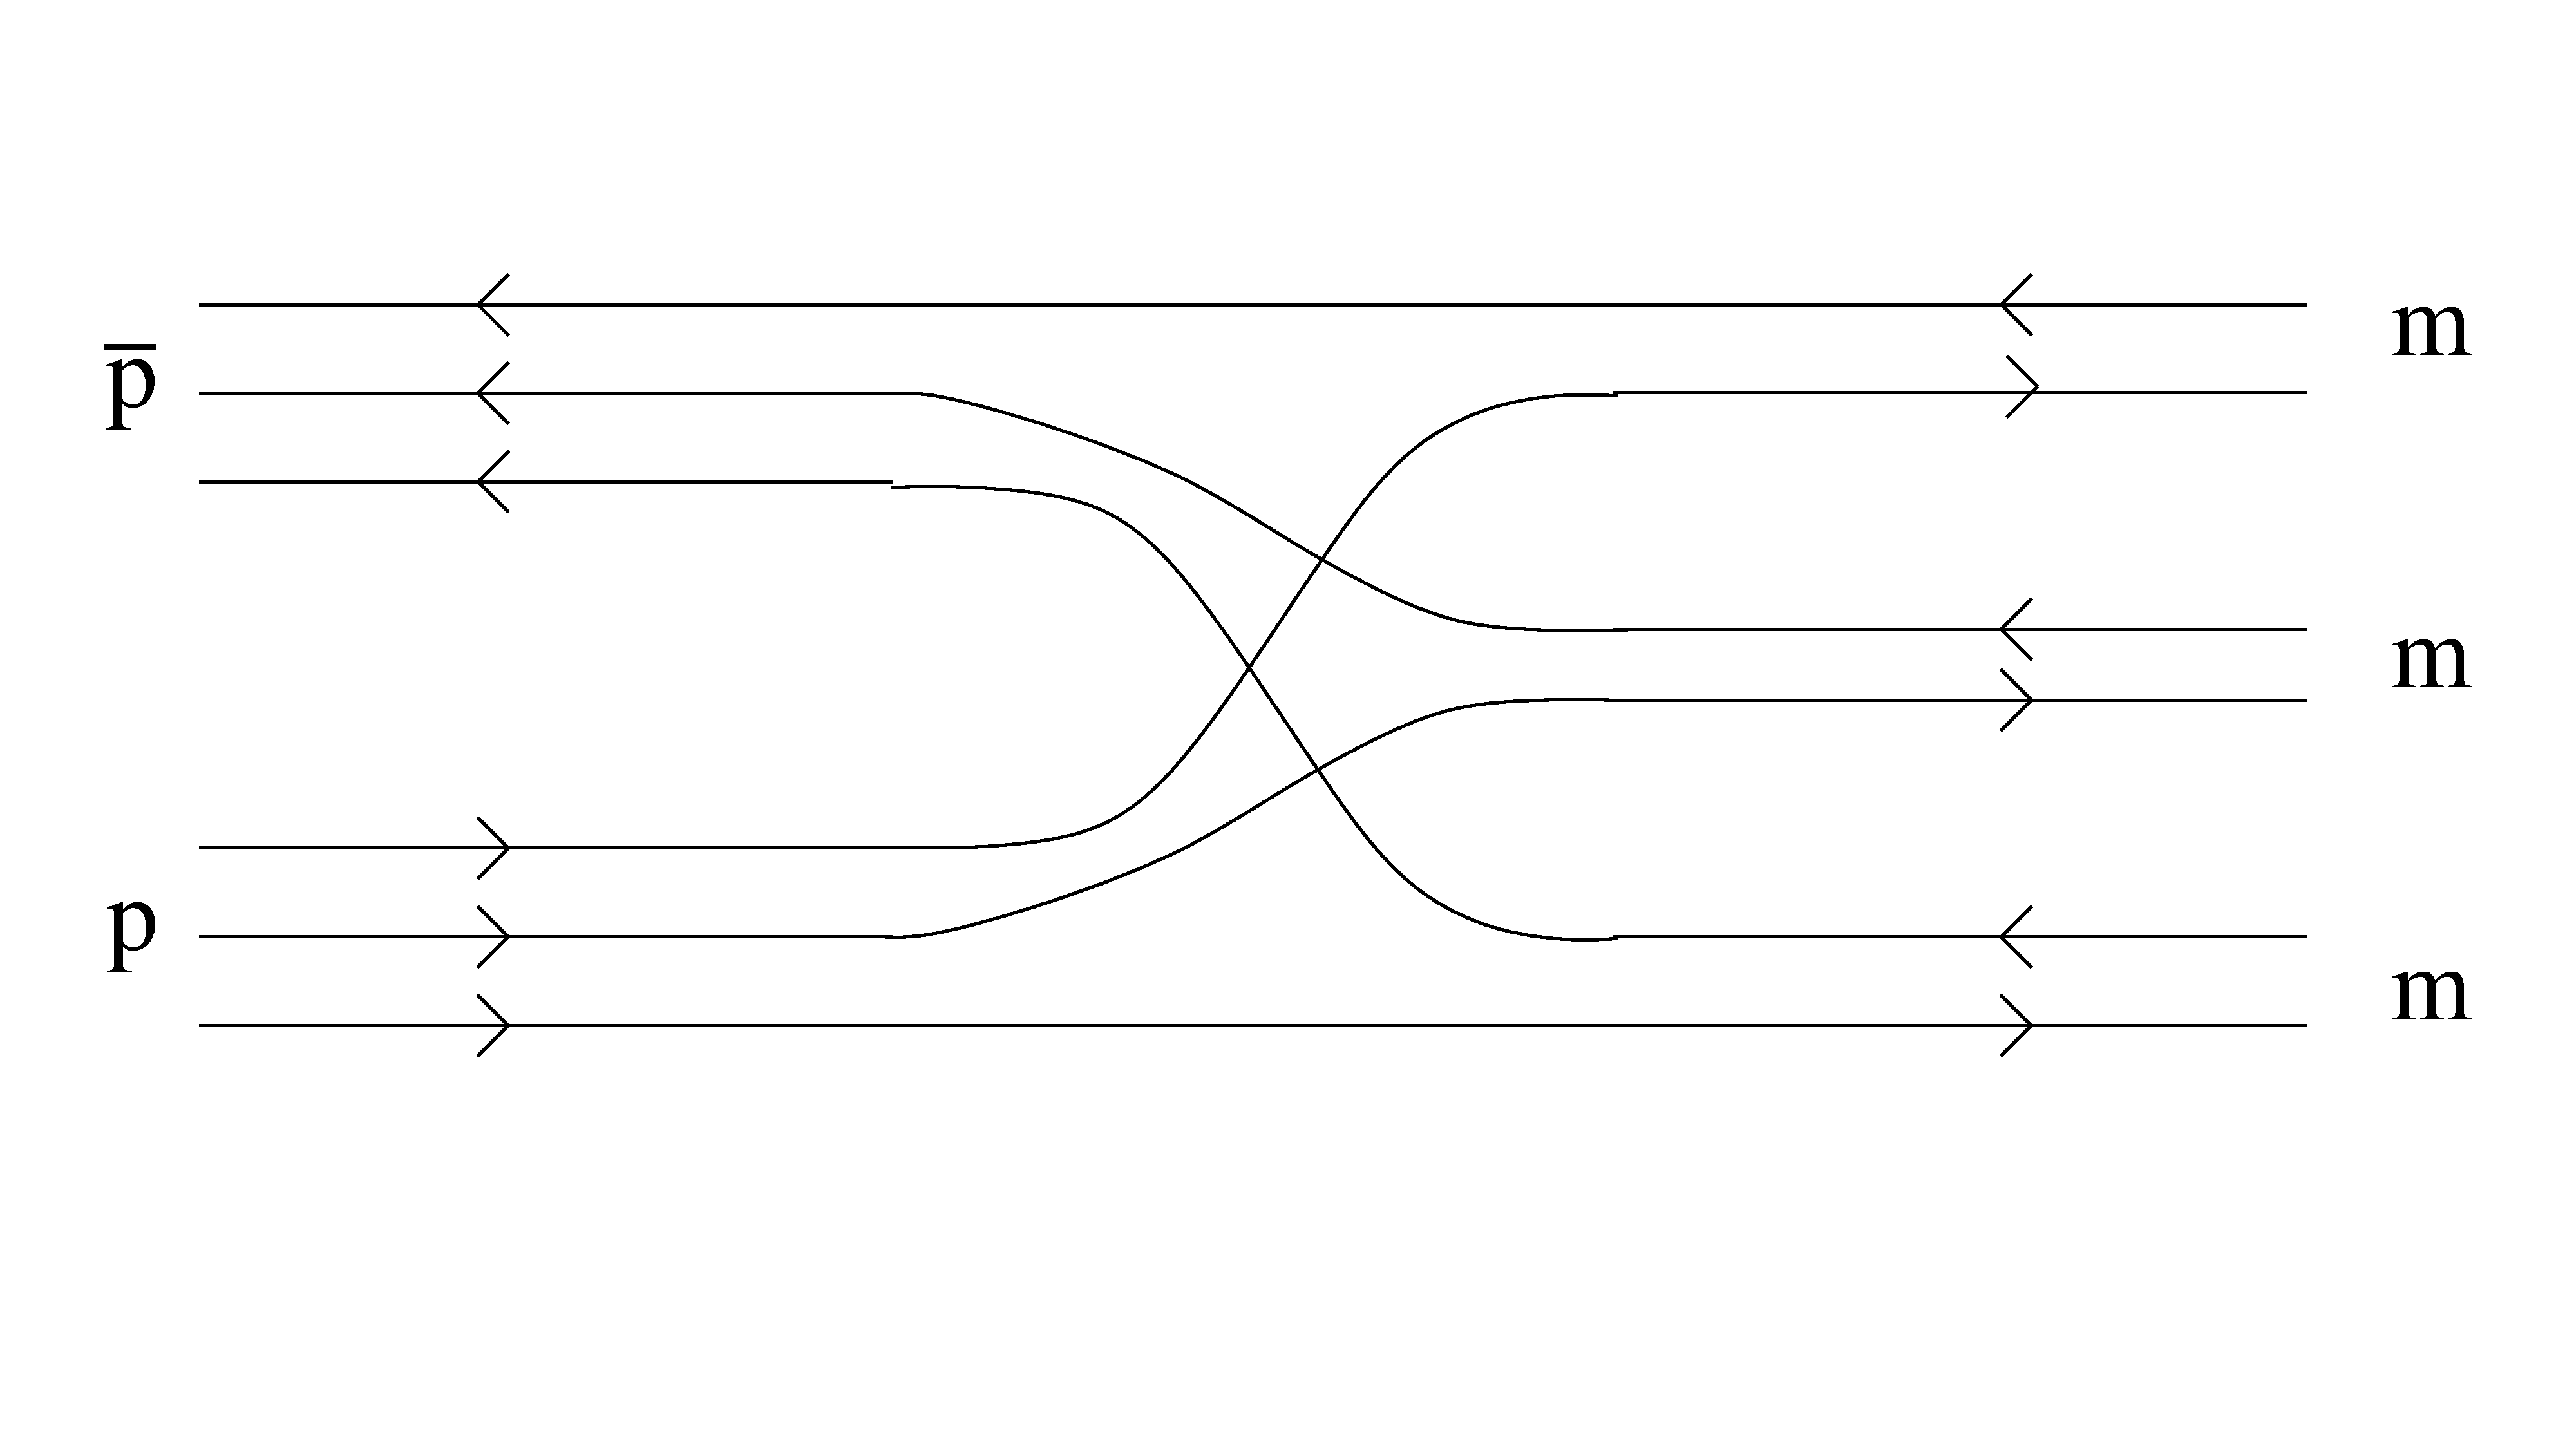
\includegraphics[width=0.9\textwidth]{figures/quark_rearrangment.pdf}
    \caption{Schematic of $\matrm{p\bar{p}}$ annihilation into 3 mesons, done by rearranging the valence quarks but without annihilating any quark-antiquark pair.}
    \label{fig:Quark_Rearrangement}
\end{figure}

%This is further complicated by the fact that due to the release of significant energy, multiple further mesons may be formed by strong fragmentation in either of these reactions. 
One important observable to distinguish between these two different annihilation mechanisms is the production of strangeness, i.e. by the reaction $\mathrm{p\bar{p}} \rightarrow 2\mathrm{K}+ X\mathrm{M}$. This reaction cannot occur with a simple rearrangement of quarks\footnote{Neglecting quark-antiquark creation by string fragmentation.}, as a new $s\bar{s}$ pair has to be created. If antiproton-proton annihilation would be dominated by the rearrangement of quarks, we would expect to see almost no produced kaons, while if the quark annihilation channel would dominate, we would expect to produce Kaons almost as much as pions. In fact we observe about 5\% of final states which include kaons\cite{antiproton_cross_sections_review, hidden_Strangeness}, suggesting that the truth lies somewhere in between the two models. \\

Given these considerations, the antiproton-proton annihilation cannot easily be described by perturbative QCD, and we are still missing an effective model capable of explaining the data. This is what makes an effective model of this interaction so difficult. Instead, an empirical parameterization is commonly used to describe the antiproton-proton inelastic cross section. A description accurately fitting the available data has been proposed by Tan et al. \cite{Tan_1983}, and is reproduced in equation \ref{eq:Talpbarpxs}, where $T_\bar{p}$ is the antiproton kinetic energy in the proton rest frame. 
%

\begin{equation}\label{eq:Talpbarpxs}
    \sigma_\mathrm{inel}^{p\bar{p}} = 24.7 (1 + 0.584T_{\bar{p}}^-0.115 + 0.856 T_{\bar{p}}^{-0.566}) \mathrm{mb}
\end{equation}

Another description -- which is implemented in the propagation code Geant4 -- is based on attempting to assign cross sections to each individual process which might occur and is explained in \cite{antiproton_dynamics_CERN}. In their model, they split the antiproton-proton annihilation into the sub processes laid out in figure \ref{fig:antiproton_annihilation_channels}. The momentum dependence of these processes is given by Regge theory \cite{antiproton_dynamics_2, antiproton_dynamics_CERN, Regge1959}. This method works for determining the cross sections into particular channels, which is necessary for an accurate description of particle propagation, as is shown in figure \ref{fig:pbar_p_xs_data_comp}. However, the description does not manage to describe experimental data better than within a factor 2. This highlights the difficulties in accurately describing the inelastic cross section of antiproton-proton annihilations.

\begin{figure}
    \centering
    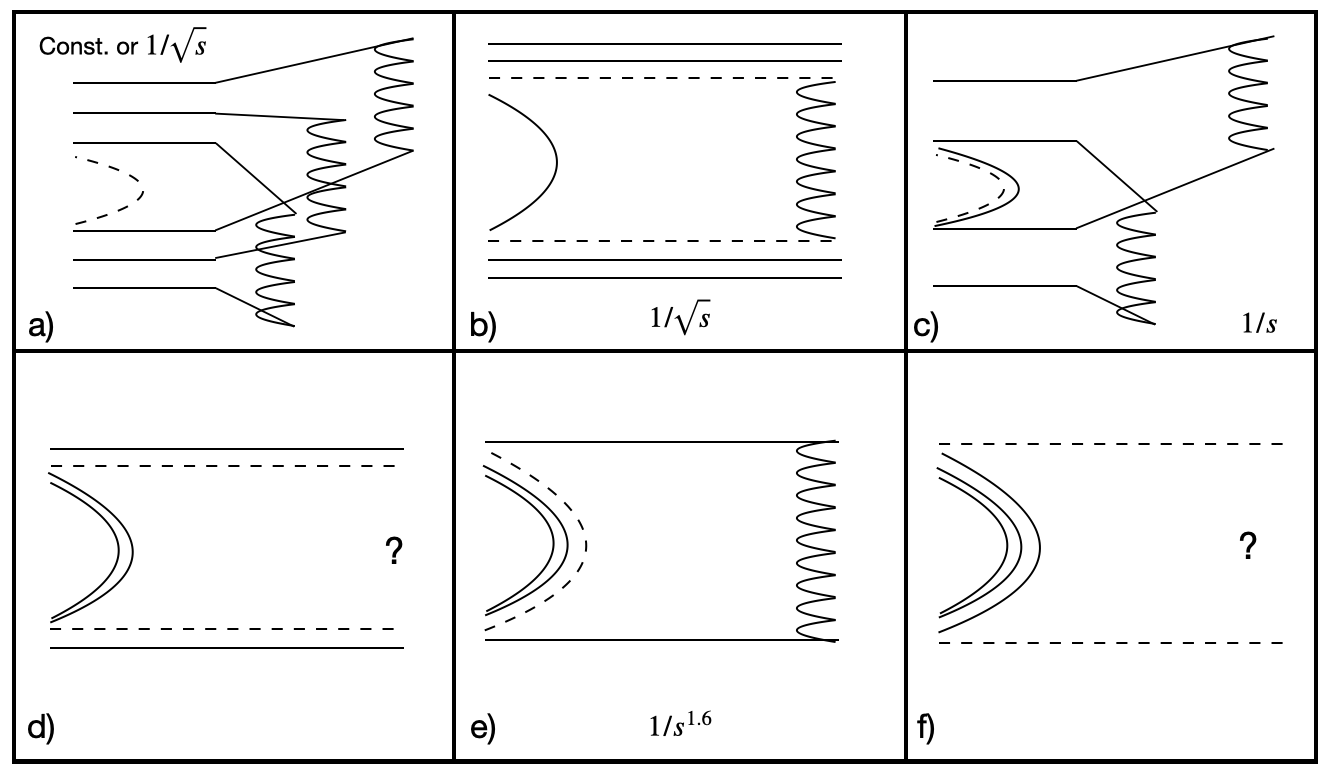
\includegraphics[width=0.6\textwidth]{figures/pbar_p_annihilation_channels.png}
    \caption{Annihilation channels for antiproton-proton annihilation. The solid lines represent quarks and the dashed lines represent a gluonic string (which can then decay via string fragmentation, as shown in figure \ref{fig:IntroStringFragmentation}). Curled lines represent a $\bar{q}q$ annihilation. The diagrams thus represent: a) 3 antiquark-quark annihilations; b) a single antiquark-quark annihilation into 2 mesons and a gluon string; c) Corresponds to a quark-antiquark and string annihilation, with the creation of 2 quark-antiquark strings. Diagrams e) and f) can produce exotic mesons. Figure taken from \cite{antiproton_dynamics_2}. \textit{This is unfortunately the highest quality figure available for this. I am planning to remake this figure in higher resolution.}}
    \label{fig:antiproton_annihilation_channels}
\end{figure}
\begin{figure}[h!]
    \centering
    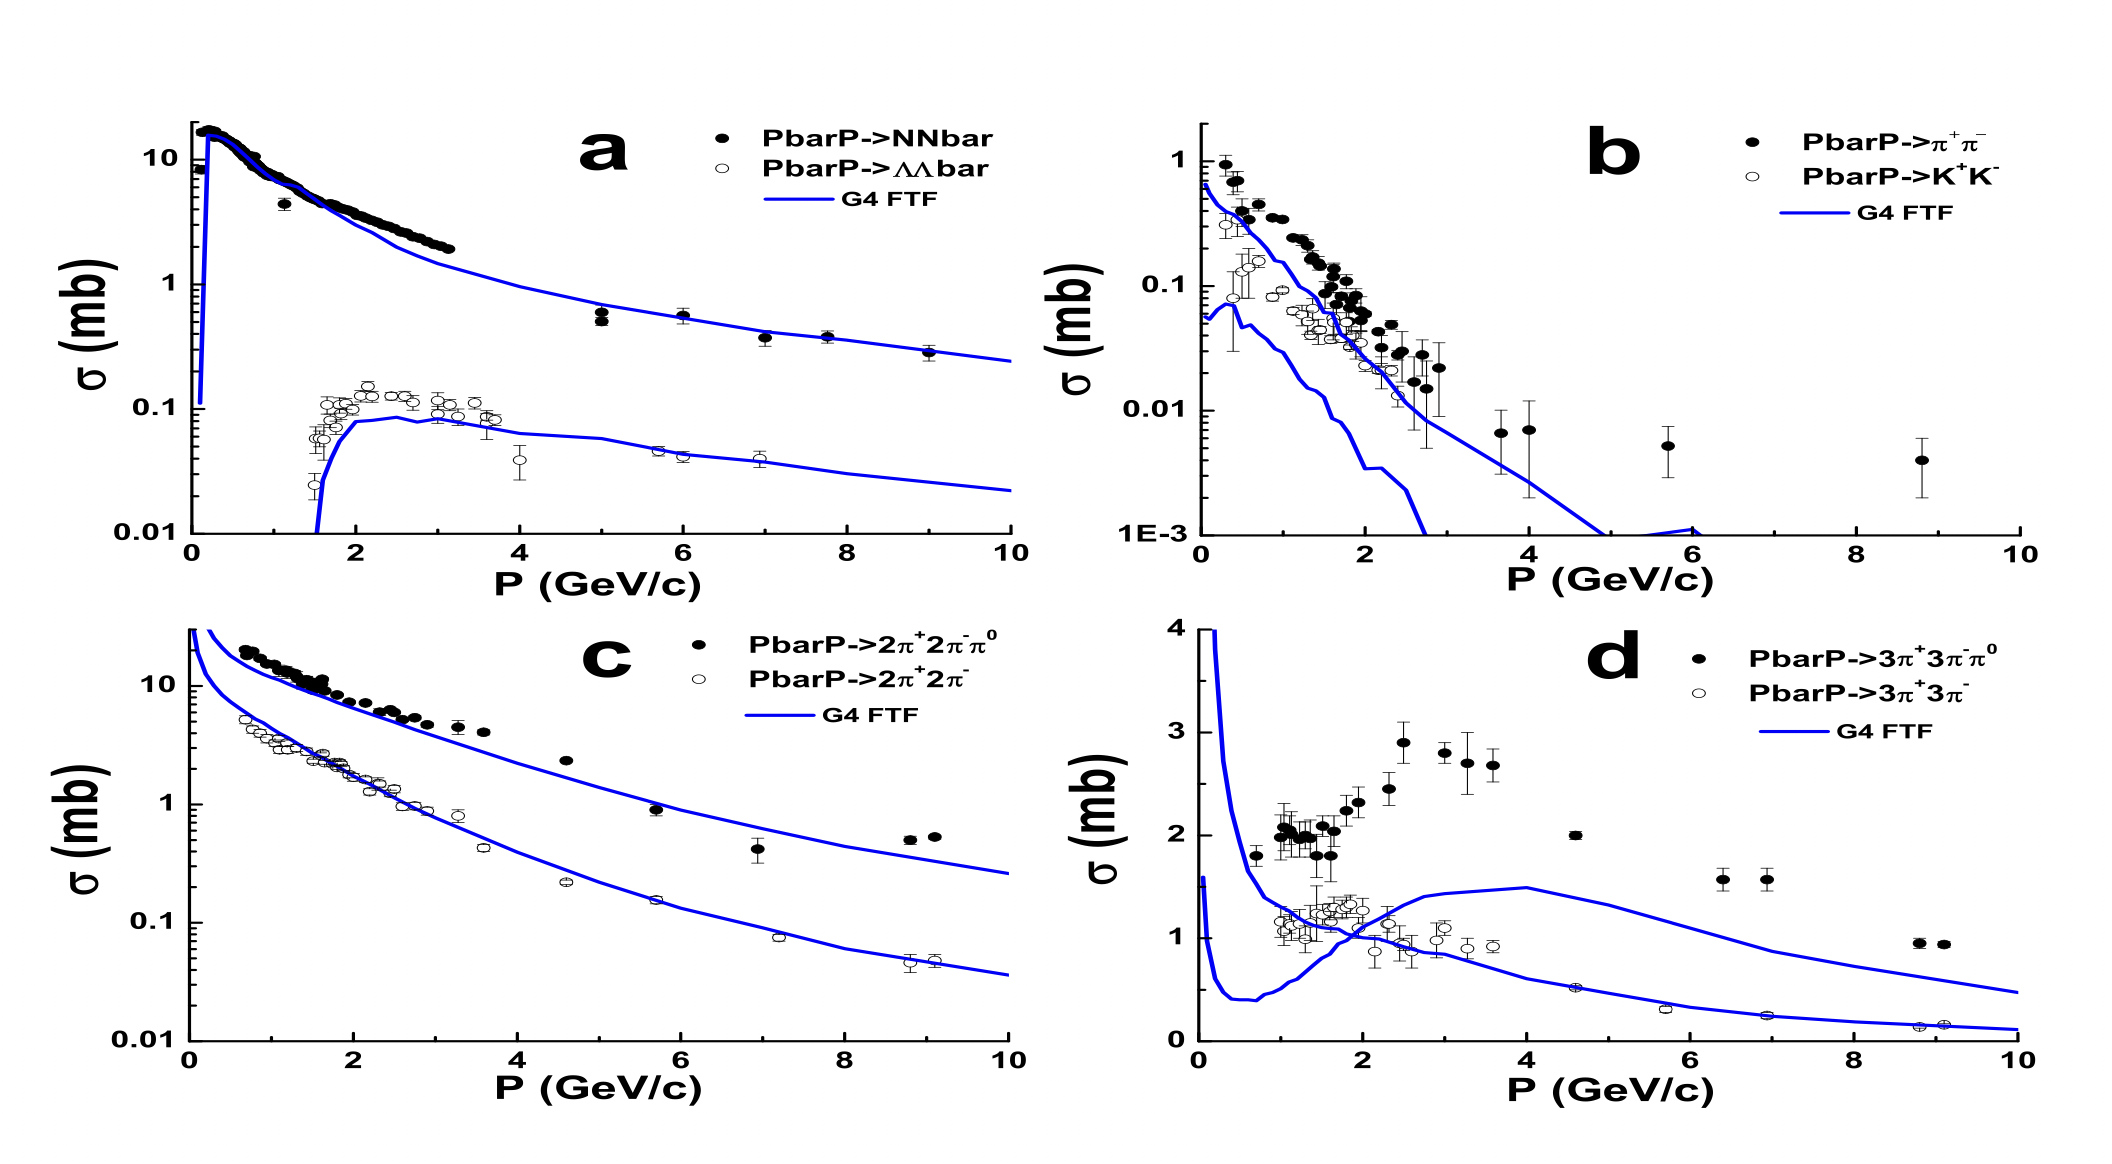
\includegraphics[width=\textwidth]{figures/Geant4_pbar_inel.png}
    \caption{A comparison of antiproton-proton inelastic cross section data with the model used in Geant4 \cite{antiproton_dynamics_CERN}. Points are experimental data as described in \cite{pbar_data}, the blue line represents the model.}
    \label{fig:pbar_p_xs_data_comp}
\end{figure}
An overview of available data on the antiproton-proton annihilation data is given in \cite{hidden_Strangeness, antiproton_physics_data, pbar_data}.



\subsubsection{Antiproton-nucleus annihilation: the Glauber model}
In the previous section it has been established that while the antiproton-proton inelastic cross section has been well measured, a theoretical description is still lacking. In this section we therefore focus on the experimental results for antiproton-matter annihilations, and how we can use them to infer something about the underlying annihilation mechanism. \\

When moving from antiproton-proton to antiproton-nucleus annihilations, several new effects come into play. The question is if only one nucleon in the nucleus interacts in the initial annihilation, and then how the antinucleus acts after the annihilation occurs. Thankfully, while those points certainly raise additional difficulties in finding a theoretical description, we can benefit from plentiful measurements of antiproton absorption on matter. These are parameterised according to the Glauber model \cite{Glauber_original, glauber_model_geant4_scaling, Antinucleus-nucleus_Geant4}. The Glauber model parameterises the inelastic cross section of antiprotons on nuclei as a geometric scaling of the antiproton-proton cross section, according to equation \ref{eq:Glauber_singleA}, where $R_A$ is a free parameter which can be roughly understood as the target nucleus' radius, and characterised as $R_A = r_0 A^{1/3}f(A)$. $r_0=1.1$ fm, and $0.8<f(A)<1.1$ is a correction factor as a function of $A$. $h$ denotes the hadron in question, $A$ is the mass number of the target nucleus and $\sigma_{hN}^{tot}$ is the total antiproton-nucleon cross section. 

\begin{equation}\label{eq:Glauber_singleA}
    \sigma_{hA}^{in} = \pi R_A^2 \mathrm{ln}\left[ 1+\frac{A\sigma_{hN}^{tot}}{\pi R_A^2}\right]
\end{equation}

\begin{figure}
    \centering
    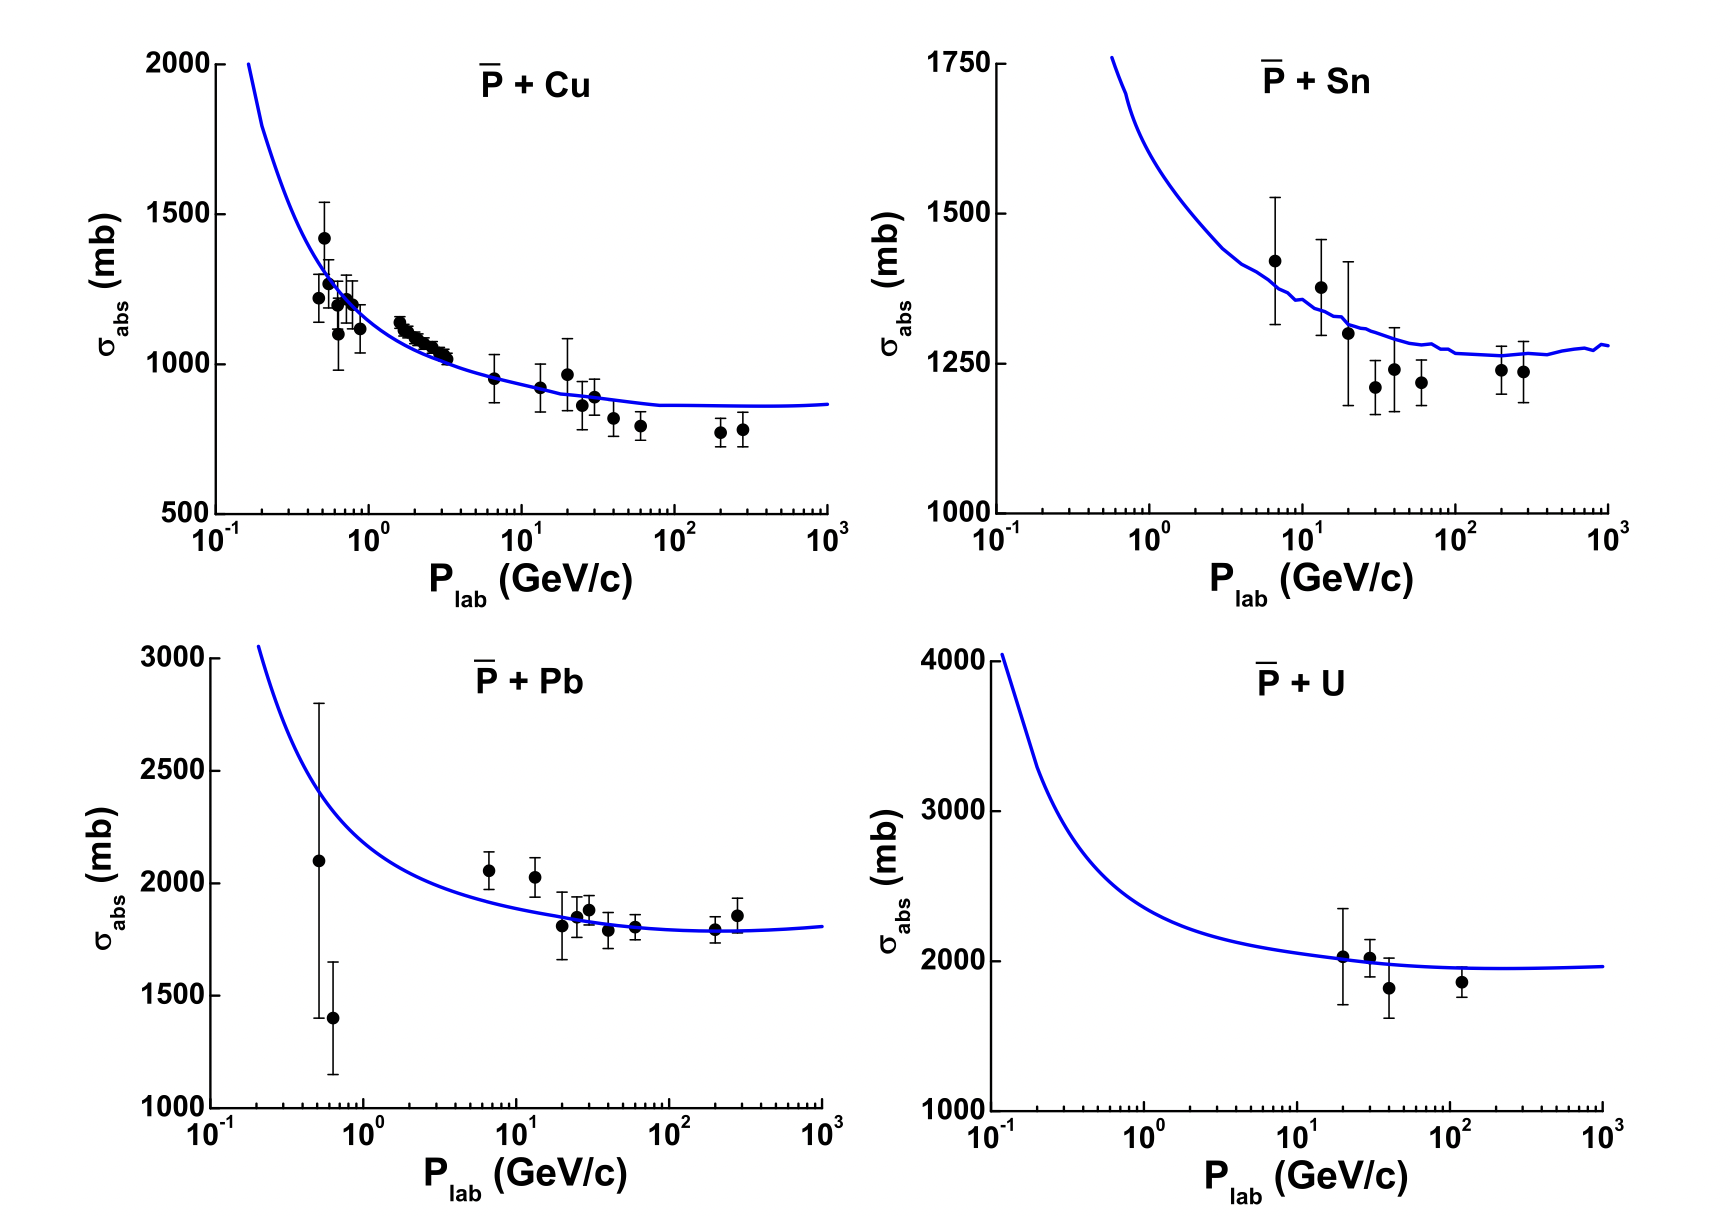
\includegraphics[width=0.9\textwidth]{figures/pbar_annihilation_diff_materials.png}
    \caption{Antiproton-nucleus annihilation for different materials, taken from \cite{Antinucleus-nucleus_Geant4}.}
    \label{fig:pbar_diff_materials}
\end{figure}


\subsubsection{Antinuclei-matter annihilations: the Glauber model and geometric scaling}\label{sec:IntroGlauber}
Having established the details of the antiproton inelastic cross section, we can now start to consider the process of antinuclei annihilation. All the considerations made for the antiproton inelastic cross section still hold true, but additionally there is also the potential between the antinucleons to consider. This means that one not only has to consider the breakup of the matter nucleus, but also the breakup of the antimatter nucleus, leaving a smaller antinucleus behind. This has been observed for antideuterons in the reaction $\overline{\mathrm{d}} + A \rightarrow \overline{\mathrm{p}}+X$\cite{Denisov:1971im, Binon:1970yu}. However, it is not clear if the antiproton which was measured survived the initial collision or if it was created from the annihilation of the antideuteron.\\

In order to scale up the cross sections from antiproton-nucleus to antinucleus-nucleus annihilations, we can also employ the Glauber model. The full mathematical treatment can be found in \cite{Uzhinsky:2011zz}, however, due to the computational effort required to do real time Glauber calculations, Geant4 uses a parameterization to approximate the result of Glauber calculations. This parameterization is based on extending \ref{eq:Glauber_singleA} to light antinuclei, according to equation \ref{eq:Glauber_multA}, where $B$ is the mass number of the antinucleus. 

\begin{equation}\label{eq:Glauber_multA}
     \sigma_{BA}^{in} = \pi(R_A^2+R_B^2) \mathrm{ln}\left[ 1+\frac{BA\sigma_{hN}^{tot}}{\pi ( R_A^2 + R_B^2)}\right]
\end{equation}

$R_A$ is then used as a fit parameter to tune the simplification to the expected value of full Glauber calculations. The form of $R_A$ is given by equation \ref{eq:RA}:

\begin{equation}\label{eq:RA}
    R_A = c_1 A^{0.21}+c_2 A^{1/3}
\end{equation}
, where $c_1$ and $c_2$ are constant whose exact value depends on the antinucleus on question. The values are given in table \ref{tab:antinucleus_nucleus_constants_Glauber} for the antinuclei up to $A=4$. 

\begin{table}[]
    \centering
    \begin{tabular}{|c|c|c|}
        \hline
        antinucleus & $c_1$ & $c_2$ \\
        \hline 
        $\overline{\mathrm{p}}$& 1.31& 0.9\\
        \hline
        $\overline{\mathrm{d}}$& 1.38& 1.55\\
        \hline
        $^3\overline{\mathrm{He}}$/ $^3\overline{\mathrm{H}}$& 1.34& 1.51\\
        \hline
        $^4\overline{\mathrm{He}}$& 1.30& 1.05\\
        \hline
    \end{tabular}
    \caption{Constant values for determining the fir parameter $R_A$ used in the Geant4 Glauber approximation for antinucleus-nucleus collisions. \cite{Antinucleus-nucleus_Geant4}}
    \label{tab:antinucleus_nucleus_constants_Glauber}
\end{table}




%\subsubsection{The effect of the coulomb interaction on antinuclei-matter annihilations}
%So far, only the effect of the strong force on the cross sections of antinuclei-nuclei annihilations has been considered, but there is also an electromagnetic component, since both particles are oppositely charged. 


%\subsection{Matter and antimatter in the universe}

\subsubsection{Origin of hadronic matter}

\subsubsection{A matter dominated universe: antimatter-matter asymmetry}

\subsection{Antimatter-matter annihilations}
    
\subsubsection{Antiproton-matter annihilations on different materials}
\subsubsection{Antinuclei-matter annihilations: the Glauber model and geometric scaling}\label{sec:IntroGlauber}
\subsubsection{The effect of the coulomb interaction on antinuclei-matter annihilations}

%\subsection{Antinuclei in the cosmos}

\subsubsection{ Why producing antinuclei is so difficult: production mechanisms of antinuclei}\label{sec:IntroProductionAntinuclei}
\begin{equation}\label{eq:CoalescenceParameter}
    B_N = E_A \frac{d^3 N_A}{dp^3_A} \left[ \left( E_{p,n} \frac{d^3 N_{p,n}}{dp^3_{p,n}} \right)^A |_{\vec{p}_p=\vec{p}_n=\vec{p}_A/A } \right]^{-1}
\end{equation}
\subsubsection{ Why to we care: antinuclei as a golden channel for new physics}\label{sec:Intro:AntinucleiGoldenChannel}
The main reason why cosmic ray antinuclei make such an interesting probe for new physics is twofold: i) the rarity of the standard model processes which produce them means that any signal does not have to contend with a copious background and ii) that there are already viable theories of new physics -- namely WIMP dark matter -- which predict a detectable antinuclei signal. This has led to the coining of cosmic ray antinuclei as a "smoking gun" for new physics. 
%write about the history of the search for antinuclei

\subsubsection{ What affects antinuclei in cosmic rays: production, propagation and annihilation}
\subsubsection{ How can antinuclei in the cosmos be detected: AMS, GAPS, cubesats}

\subsection{Antinuclei in the cosmos}

\subsubsection{ Why producing antinuclei is so difficult: production mechanisms of antinuclei}\label{sec:IntroProductionAntinuclei}
The difficulty in producing antinuclei is not just due to the necessary energy to create them, but also due to their production mechanism. \\

The exact production mechanism for composite antinuclei in high energy particle collisions is still unknown. There are currently two models aiming to describe this phenomenon. The first is the statistical hadronization model, which models the production of the nuclei as a statistical process with a characteristic temperature (at heavy ion collisions at the LHC this temperature is 156 MeV \cite{4He_PbPb}). This model has had great success by describing particle yields over 9 orders of magnitude in yield, as is shown in figure \ref{fig:Stat_Hadron_model}.

\begin{figure}
    \centering
    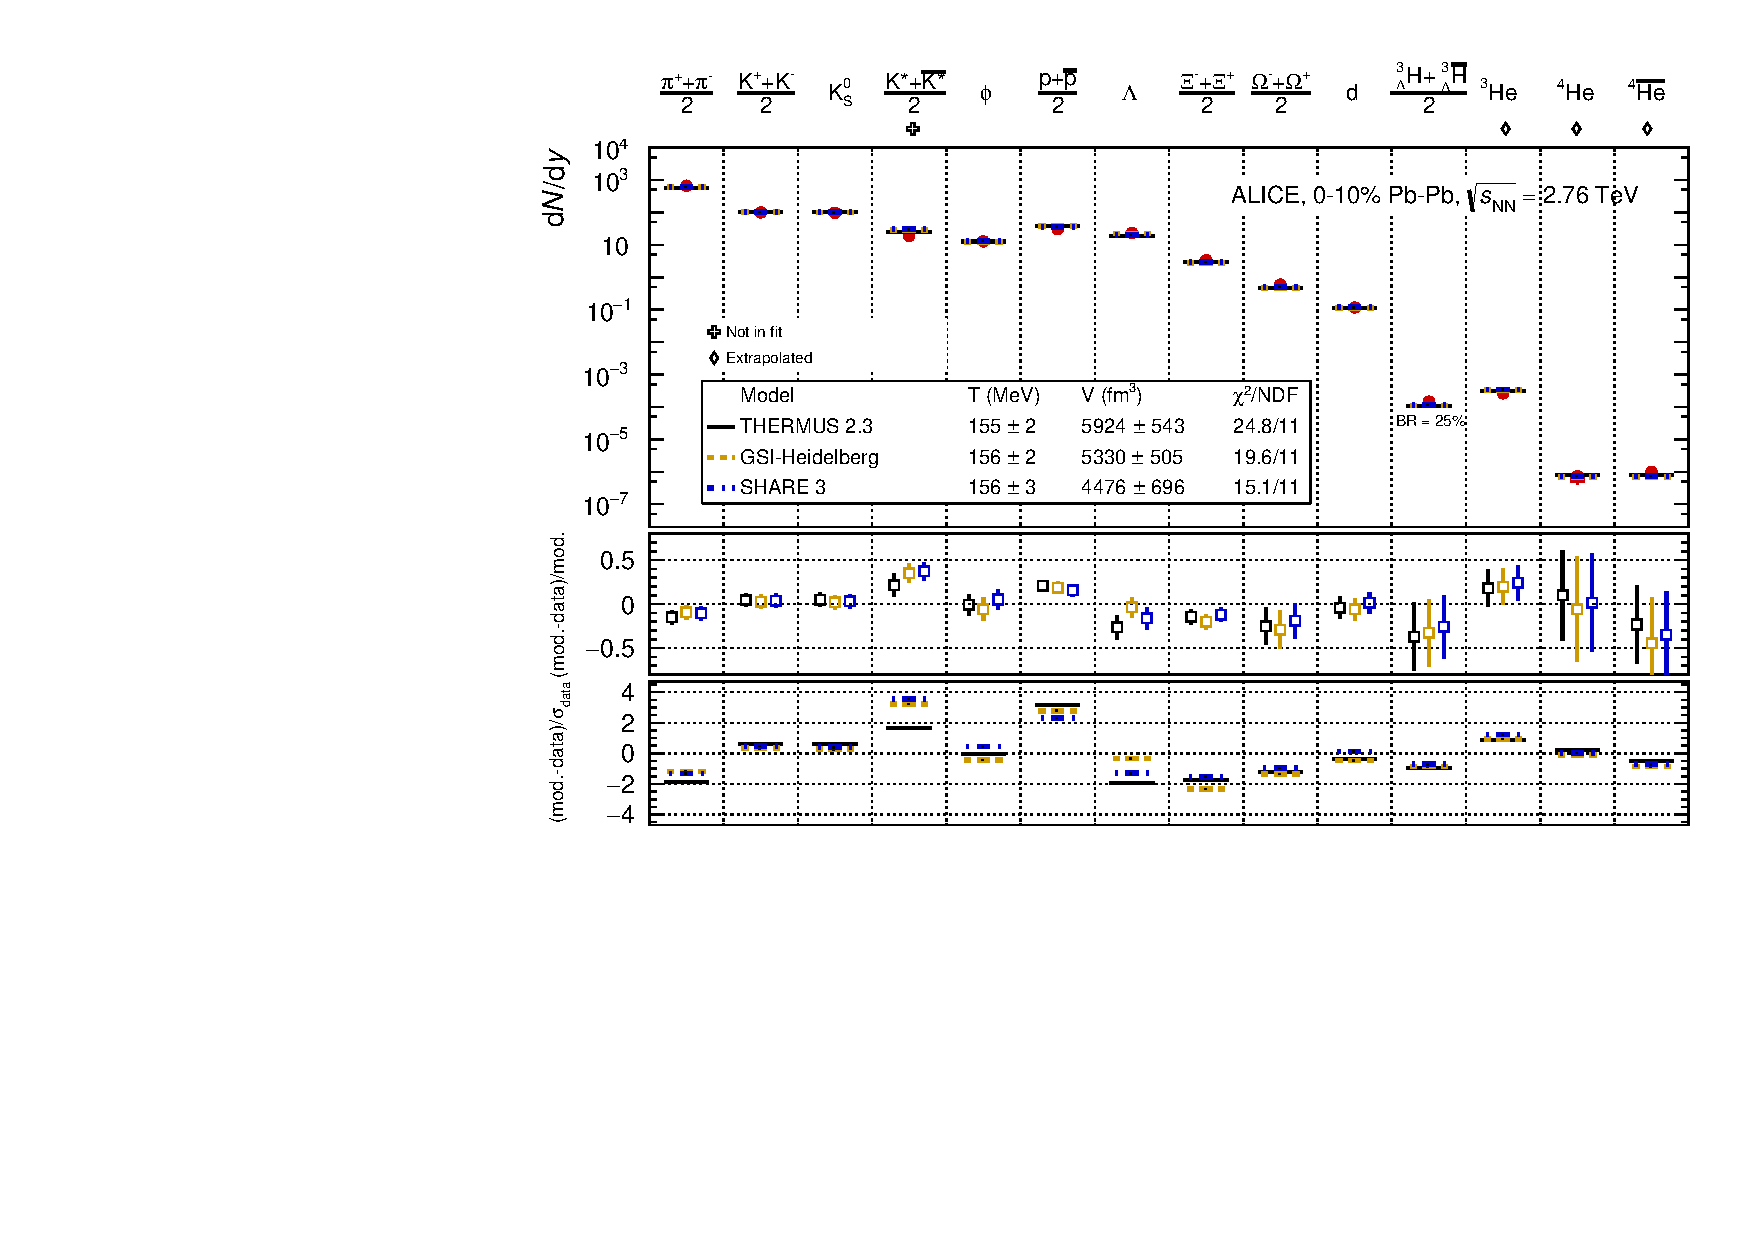
\includegraphics[width=0.75\textwidth]{figures/Fit_PbPb0010_GSITHERMUSSHARE_new_alpha_fixed-91746.pdf}
    \caption{Statistical hadronisation model fits, with three different implementations, to the light flavour hadron yields in central (0-10\%) Pb--Pb collisions at $\sqrt{s_{NN}}$= 2.76 TeV. The data points are taken from  and details of the fits can be found in . The upper panel shows the fit results together with the data, whereas the middle panel shows the difference between model and data normalised to the model value and the lower panel the difference between model and data normalised to the experimental uncertainties. Figure and caption taken from \cite{4He_PbPb}.}
    \label{fig:Stat_Hadron_model}
\end{figure}

The problem with the statistical hadronization model is that it predicts a the production of nuclei from a thermalized medium, when the binding energy of the nuclei is far below the temperature given by the model. For example, the deuteron binding energy is $\approx 2.2$ MeV, compared to the temperature of 156 MeV predicted by the model. This has been dubbed the "snowball forming in hell" problem. Additionally, the statistical hadronisation model says nothing about the underlying mechanism by which the nucleons form antinuclei. \\

The second model is the coalescence model. This model considers the relative momenta of nucleons produced in the collision, and if they are close enough together, assigns them a chance to bond together and form a nucleus. The advantage of this is then that given a set of space and momentum coordinates\footnote{Traditionally coalescence models neglect the spatial correlation part, assuming that the nucleons are close enough together in space to coalesce. And any difference between the sizes of collision systems is then accounted for by a different coalescence parameter.}, the coalescence model can predict the nuclei spectra from the spectra of protons and neutrons. This relation is then experimentally characterized by equation \ref{eq:CoalescenceParameter}:

\begin{equation}\label{eq:CoalescenceParameter}
    B_A = E_A \frac{d^3 N_A}{dp^3_A} \left[ \left( E_{p,n} \frac{d^3 N_{p,n}}{dp^3_{p,n}} \right)^A |_{\vec{p}_p=\vec{p}_n=\vec{p}_A/A } \right]^{-1}
\end{equation}
, where $B_A$ is the coalescence parameter. While this model also requires fits to experimental data in order to give predictions of the yields and spectra of antinuclei, it gives an explanation for the mechanism of how nucleons bond together. For a more comprehensive review of the coalescence model, see \cite{Kachelriess:2020uoh, Coalescence2015}.\\

What can we infer from these models on the production of antinuclei? The important takeaway for this thesis is that their production relies on significant amounts of available energy, and on producing two nucleon close in both space and momentum. These restrictions limit the production of antinuclei to high energy collisions or exotic production channels.

\subsubsection{ Why to we care: antinuclei as a golden channel for new physics}\label{sec:Intro:AntinucleiGoldenChannel}
The main reason why cosmic ray antinuclei make such an interesting probe for new physics is twofold: i) the rarity of the standard model processes which produce them means that any signal does not have to contend with a copious background and ii) that there are already viable theories of new physics -- namely WIMP dark matter -- which predict a detectable antinuclei signal. This has led to the coining of cosmic ray antinuclei as a "smoking gun" for new physics. \\

The first discovery of antimatter in cosmic rays was also the first discovery of antimatter in general: the discovery of the positron in charged particle showers from cosmic rays, in 1932 \cite{positron_discovery}. The discovery of antiprotons in cosmic rays would take almost half a century more, finally being observed in 1979 \cite{antiproton_CR_discovery, Bogomolov:1979hu}. During this time, antiprotons in cosmic rays were a probe into the matter-antimatter asymmetry of the universe, as their abundance could give a hint to the presence of antimatter dominated regions in our galaxy. Their discovery and study to the present day are consistent within uncertainties with production from high energy collisions of cosmic rays with the interstellar medium, providing no evidence for any antimatter dominated regions\footnote{Nowadays constraints on antimatter dominated regions are more stringently set by gamma ray searches.}. The antiproton to proton ratio in cosmic rays is roughly $10^{-4}$. \\

Nowadays, the focus is on the search for antinuclei as a probe of new physics. The expected production from high energy cosmic ray collisions is very low, particularly at low energies (see section \ref{sec:AntinucleiInTheCosmos} for exact values), while several dark matter models predict an antinuclei flux within reach of current or next generation detectors\cite{Doetinchem_2020_review}. The antinuclei of interest are antideuterons and $^3\overline{\mathrm{He}}$. Even though the former is expected to be produced in much greater amount, the same charge and similar mass to the proton make a discrimination harder as for $^3\overline{\mathrm{He}}$, being a charge $Z=-2$ particle. For both, the background in the low energy region (below a few GeV/nucleon) is expected to several orders of magnitude below the expected signal strength. This is in strong contrast to searches involving gamma rays \cite{}, or antiprotons \cite{}, where the signal to background ratio is expected to be on or below the \% level. Thus, an observation of a low energy antinuclei flux would be a sign for new physics. 
%write about the history of the search for antinuclei

\subsubsection{ What affects antinuclei in cosmic rays: production, propagation and annihilation}
As explained in the previous section, low-energy antinuclei in cosmic rays provide a uniquely background free probe into new physics. But in order to interpret any future observation, it is necessary to understand what affects their abundance and spectral shape. These factors can be summed up as 3 things: their production, propagation and annihilation. While a more detailed description of each is given in section \ref{sec:AntinucleiInTheCosmos}, this section aims to give a brief introduction on the importance of the three aspects. \\

The production of antinuclei in cosmic rays can be classed into two categories: i) production in high energy collisions of cosmic rays with the interstellar medium and ii) new, exotic sources. This is different to light nuclei in cosmic rays, whose production is dominated by their production in the stellar cycle. Their production in high energy cosmic ray collisions can be somewhat constrained by experiments at accelerators, which probe fundamentally the same reaction of $p + p \rightarrow \overline{\mathrm{d}}/^3{\overline{\mathrm{He}}} + X$. However, the energies and rapidities at which production mostly occurs are usually at much lower energies than the ones probed by acclerators, e.g. for antideuterons the most important centre-of-mass energy for production in high energy cosmic rays is $\sqrt{s}\approx 25$ GeV (see figure \ref{fig:dbar_2d_source_CR}). Furthermore, the experiments most capable of studying antinuclei, the ALICE experiment at the LHC and the STAR experiment\cite{} at the Relativistic Heavy Ion Collider, probe their production at midrapaidity, rather than at the highly forward rapidities relevant for production in cosmic ray collisions. This means that for much of the relevant parameter space for production, extrapolation from experimental data is necessary. On the other hand, production from new physical processes -- such as the annihilation of WIMP dark matter which is discussed in detail in this thesis -- is even less constrained, and has to be probed by letting Monte Carlo simulations run from an assumed standard model state in the annihilation. \\

Once the antinuclei are produced, they travel through the galaxy until they eventually reach earth. On this journey they are affected by magnetic fields, bulk motion (i.e. diffusion and convection effects), as well as other effects. The good thing is that these affects are the same for all cosmic rays, and can therefore be constrained by observations of more abundant cosmic ray species. Recent work on the topic was done in \cite{Boschini:2017fxq, Boschini:2018baj}, and is explained in more detail in section \ref{sec:AntinucleiInTheCosmos}. \\

On their journey, antinuclei do not merely travel through empty space; the space between stars is filled with the diffuse interstellar medium (ISM), which is made up of about 0.9 protons per cubic centimeter \cite{}. As antinuclei traverse this matter, they might interact and annihilate with it. To account for this loss it is necessary to quantify the inelastic cross section of antinuclei down to low energies. The measurement of these cross sections and the quantification of their effect on antinuclei losses is the topic of this thesis. 
%\subsubsection{ How can antinuclei in the cosmos be detected: AMS, GAPS, cubesats}
%This is all explained towards the end of chapter 5, why rehash it here? 
\subsection{Antinuclei on earth}
On earth, we have the ability to artificially produce antinuclei at high energy physics facilities, like the LHC. In fact, antideuterons were first observed in 1965 in collisions of protons on Beryllium at the Proton Synchrotron\cite{Massam:345976}. Since then, antinuclei have been observed in higher energy collisions in much larger amounts, both at CERN facilities \cite{nuclei_pp_13TeV, nuclei_pp_5TeV, nuclei_pp_PbPb, nuclei_pp}, and heavy ion facilities \cite{}. The ALICE experiment in particular, has published spectra of antinuclei up to $^4\overline{\mathrm{He}}$ \cite{nuclei_pp_13TeV, nuclei_pp_5TeV, nuclei_pp_PbPb, nuclei_pp} in both pp and Pb-Pb collisions. This section aims to give an overview of the studies of antinuclei on earth. 
\subsubsection{Production at accelerators}
Production at accelerators can be classed by energy, and by collisions system. Energy affects the barychemical potential \footnote{The baryochemical potential is a measure of how much more energy is required to produce antibaryons to baryons. A value of 0 means that they are produced in equal amounts, and is found at LHC energies at mid-rapidity\cite{primordial_ratio1, primordial_ratio2}.}, while the collisions system determines the penalty factor for producing heavier (anti)nuclei. The penalty factor -- which describes the amount by which the production of (anti)nuclei is suppressed for each additional nucleon -- is roughly 1/300 in Pb--Pb collisions at 5.02 TeV, while being roughly 1/1000 in pp collisions at 13 TeV \cite{antinuclei_mult_dependence}. The relative $p_T$ integrated yields of nuclei are shown in figure \ref{fig:PenaltyFactorNuclei}. \\

\begin{figure}[h!]
    \centering
    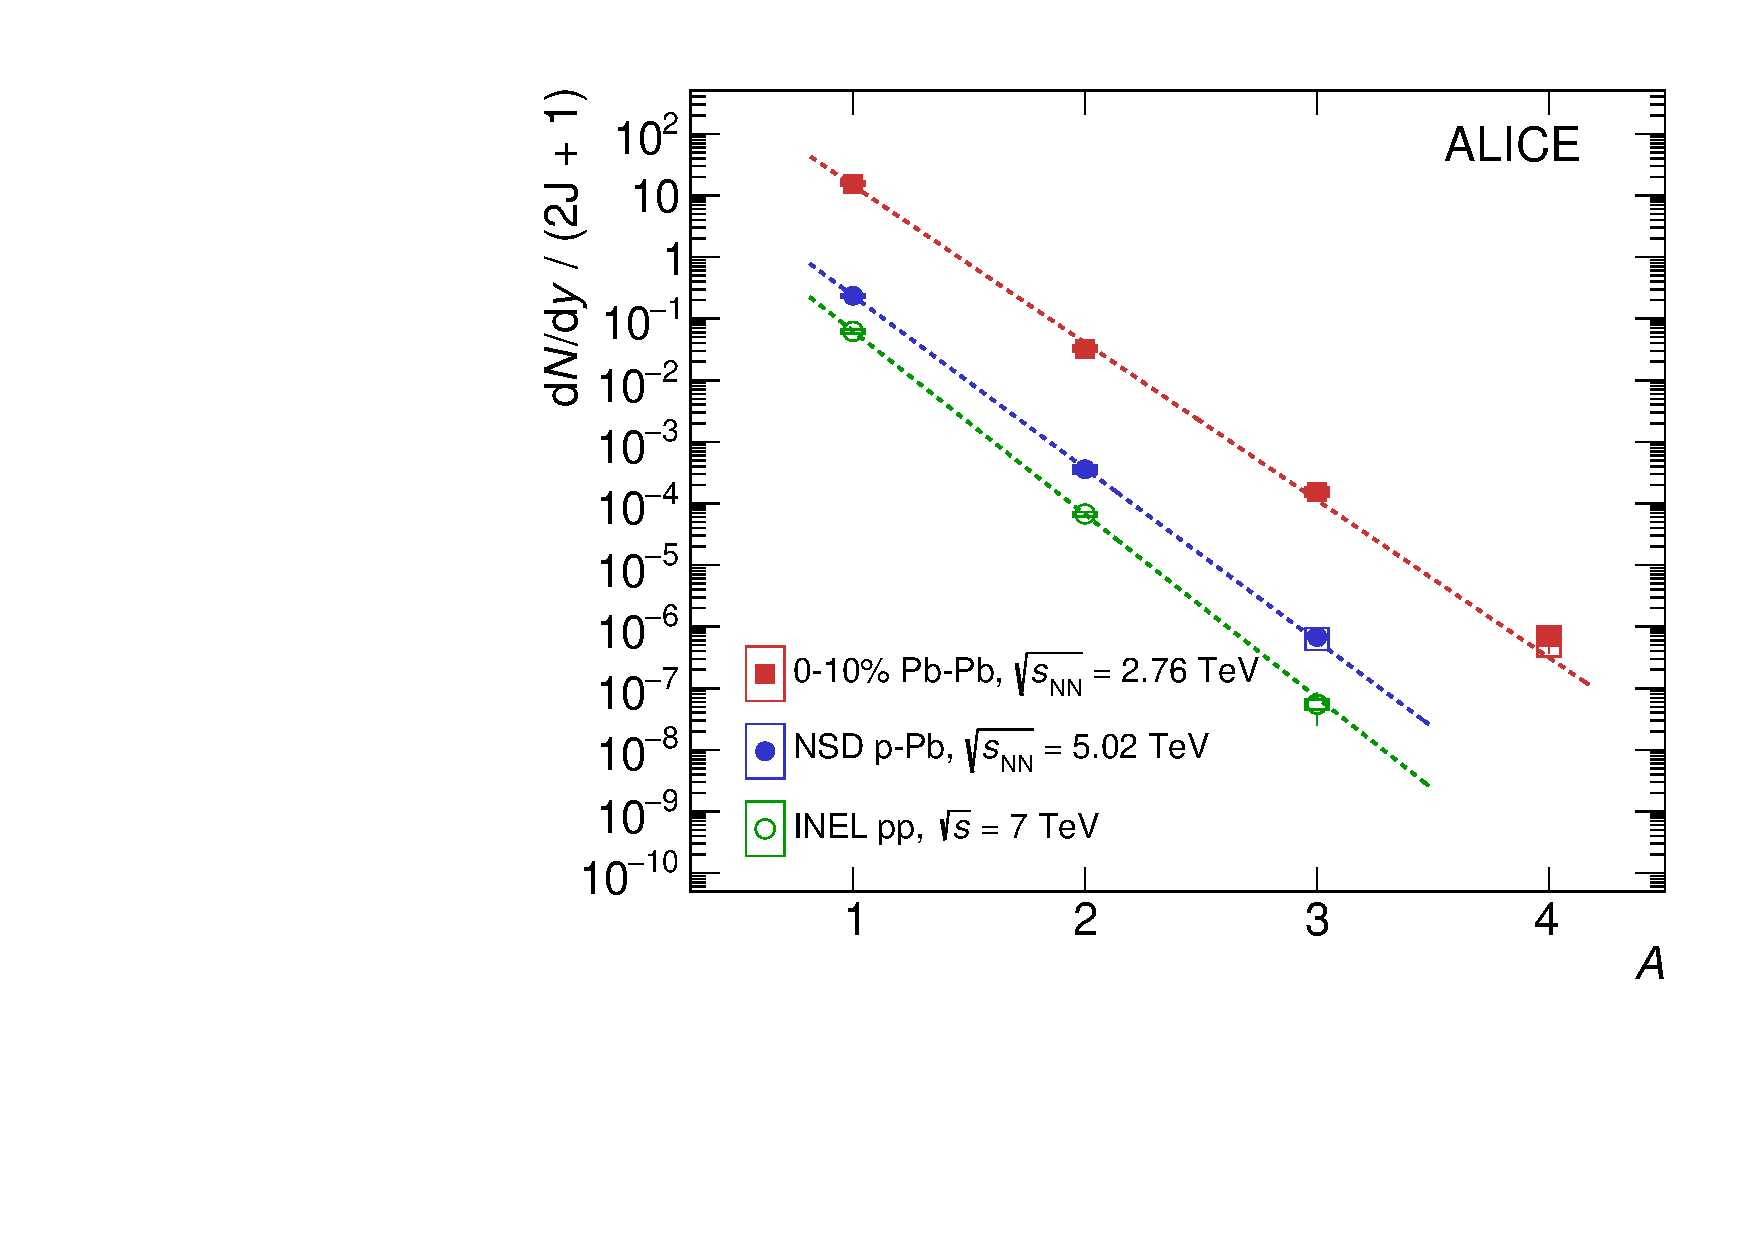
\includegraphics[width=0.8\textwidth]{figures/PenaltyFactor-97548.pdf}
    \caption{Production yield $d\mathrm{N}/dy$  normalised by the spin degeneracy as a function of the mass number for inelastic pp collisions, minimum-bias p-Pb and central Pb-Pb collisions . The empty boxes represent the total systematic uncertainty while the statistical errors are shown by the vertical bars. The lines represent fits with an exponential function. Figure taken from \cite{antinuclei_mult_dependence}.  }
    \label{fig:PenaltyFactorNuclei}
\end{figure}



\subsubsection{Annihilation at accelerators}
Traditionally, annihilations have been studied in fixed target experiments\cite{}. In those experiments, a beam of antiparticles is produced and then fired at a target. The number of particles before and after the target are measured, and the resulting disappearance probability is used to calculate the inelastic cross section. However, this method relies on the ability to produce a clean beam of antiparticles, with sufficient statistics to conduct such an experiment. This comes with two challenges: i) the difficulty of producing antinuclei due to the required energy thresholds and ii) producing the antinuclei in a focused direction, so that they can be captured directed towards a target. These two constraints are unfortunately counterproductive. In order to compensate the difficulty of meeting the energy requirement for the collisions, it is far more energetically favourable to collide in the particles rest frame, however, this produces particles in all directions, not focused towards the beam direction. This makes such measurements increasingly more difficult for higher mass antinuclei.\\

However, since antinuclei up to $A=4$ have been observed in heavy ion collisions \cite{4He_PbPb}, they also have to annihilate in the detector. But it is far more difficult to find an equivalent observable to the fixed target experiment within such an experiment, because it is a priori not possible to know how many particles get produced, and therefore the "loss" of particles is not trivial to measure. The methods developed to measure this loss are the topic of this thesis and will be explained in section \ref{sec:ExperimentAndMethod}, so just a brief introduction is given here. The first method is based on using the knowledge of nuclei production and the baryochemical potential to calculate how many antinuclei should have been produced. The second is based on measuring the particles individually in two different detector systems, and to calculate the loss between the two. 

\subsection{Dark matter and its connection to antinuclei}
In this section a brief introduction into the motivation and evidence for dark matter is given, several prominent dark matter models are discussed, with a particular focus on WIMP dark matter. Furthermore, the connection with WIMP dark matter and antinuclei is discussed. 
\subsubsection{The evidence for dark matter}
The first evidence for dark matter was observed by Zwicky \cite{Zwicky} in 1933, who realised that the rotation curves in galaxy clusters could not be caused solely by the luminous matter observed. His conclusions were not taken seriously until almost 40 years later, when the search for missing mass caused by the advent of cosmology made his theory of dark matter attractive. During this time, the big bang cosmology had prevailed, but left open the question of the ultimate fate of universe. Within big bang cosmology, there are three option. The first is that the universe expands forever, with the gravitational pull merely slowing down the expansion over time, never stopping it. The second is a closed universe, where the density of matter is bigger than some critical density, and therefore will eventually outperform the expansion, causing a collapse of the universe back towards a hot dense medium. And finally, a flat universe, where the density is exactly this critical density, such that eventually the gravitational pull of galaxies will exactly counterbalance the expansion, asymptotically reducing the expansion to 0. From Einstein's theory of general relativity, it can be shown that these fates correspond to the geometry of the universe, and are characterised by a density $\Omega$, where the critical density leading to a flat universe is given by $\Omega_c h^2= 1$\cite{PDG2022, Planck2020}. It was expected that the geometry of the universe is flat\footnote{This means that the local geometry of spacetime is euclidean, which means that all the angles in a triangle in this space add up to 180 degrees. As a counterexample to euclidean space, consider the surface of a sphere, like the surface of earth. It seems locally euclidean, when you lay a triangle on flat ground and add up the angles, they come out to 180 degrees within the measurement uncertainties. But now consider an airplane which starts at the equator flying due north to the north pole. Once it reaches there it makes a 90 degree turn, and flies due south until it once again reaches the equator. It then turns 90 degrees again so it flies along the equator back towards its original destination. The triangle made by the airplane consists of 3 90 degree angles, or 270 degrees. As such, the surface of a sphere like earth is not a euclidean space.}, but observations from galaxy clusters showed that luminous matter only made up a fraction of this density\cite{Planck2020}.%history of dark matter 
Cosmologist turned back to Zwicky's discovery \cite{history_of_dark_matter, Ostriker_return_to_DM}, claiming that dark matter made up the missing mass. \\

More evidence of dark matter was soon to follow. Tracking the rotation curve in galaxies provided evidence for dark matter bound in galaxies\cite{Sofue2020, Sofue_2016, history_of_dark_matter}. Measuring the dispersion velocities of galaxies around either other galaxies (such as the velocities of dwarf galaxies around a more massive one) or around galaxy clusters provided evidence for dark matter trapped in larger gravitationally bound structures, as did gravitational lensing\cite{Cluster_lenses}. For a comprehensive review of the evidence for dark matter see the particle data group \cite{PDG2022}. Each piece of evidence points to a type of matter which does not interact electromagnetically (hence "dark"), and makes up the majority of the mass found in cosmic structures. \\

Further evidence for dark matter can be found in structure formation in cosmology. From anisotropies in the cosmic microwave background (CMB), it can be inferred that at the time of CMB decoupling the baryonic density fluctuations were of order $\delta\rho_\mathrm{rec} / \rho \approxeq 10^{-5}$. Since these fluctuations scale linearly with the expansion of the universe, today's baryonic density anisotropies can be calculated as $\delta\rho_b / \rho |_\mathrm{today}\approxeq 10^{-2}$\cite{PDG2022}. Since matter is highly concentrated into galaxies in the present day universe, fluctuations are $\delta\rho_b / \rho |_\mathrm{obs}>> 1$. This discrepancy can be solved by adding a dominant non-relativistic, collisionless component the mix, which decoupled from thermal equilibrium well before the CMB. In other words, in order to explain structure formation from the early universe, one needs a dominant component of the mass to be in a form which does not interact electromagnetically, and does not heavily self-interact, which is also what is needed in order to explain the present-day observations of galactic motion. \\

Finally, it is important to discuss the difference between hot and cold dark matter. Dark matter which was thermally produced in the early universe -- called a thermal relic -- can be split into two categories: hot relics, which were still ultra-relativistic when they decoupled from thermal equilibrium, and cold relics, which were no longer relativistic, or cold enough to significantly cool from the expansion of the universe. Due to the different velocities of these relics, hot relics are expected to cause sharp features in the large scale structure of the universe, while cold dark matter is expected to cause a smooth large scale structure. This can be understood as how easily a particle is trapped in a gravitationally collapsed structure. After an initial overdense region forms and a gravitational well builds, slow (cold) particles will be trapped in the well first, while fast (hot) particles will not be trapped in the well until the gravitational well becomes much deeper. To get an idea of the order of magnitude of velocities, consider the escape velocity of our galaxy, which lies around 600 km/s \cite{MW_escapeVel}, which is equivalent to $\beta \approxeq 2 \times 10^{-3}$. Thus, relativistic particles would provide a counterbalance to the formation of gravitationally collapsed structures, and thus require deeper wells for large scale structures to form. This feature can be seen in \ref{fig:LargeScaleStructure}, which shows that the large scale structure of our universe prefers the cold dark matter model. 

\begin{figure}[h!]
    \centering
    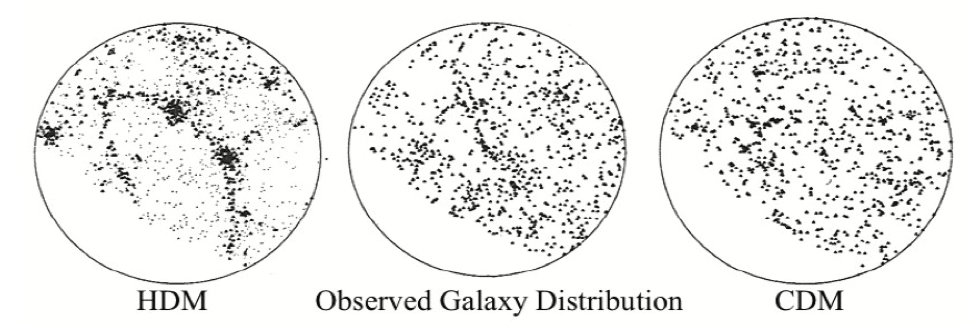
\includegraphics[width=\textwidth]{figures/Galaxy_distributions_by_DM_type.png}
    \caption{Computer simulations of the distribution of galaxies within our universe, with hot dark matter (left) and cold dark matter (right), compared to the observed distribution (middle). Figure is taken from \cite{Ibarra_neutrinos}. }
    \label{fig:LargeScaleStructure}
\end{figure}


\subsubsection{WIMP dark matter and the WIMP miracle}\label{sec:IntroWIMPs}
WIMP dark matter is candidate model for dark matter, which explains dark matter as heavy particles which only interact gravitationally an through the weak force. WIMPs are a tempting choice for dark matter, since their properties could explain all the observed phenomena (galactic motion and structure formation). A WIMP is a stable particle\footnote{The WIMP lifetime must be greater than the current age of the universe, since otherwise most would have decayed by now.}, with a mass from a few GeV to a few TeV. At their inception there were several promising WIMP candidates from supersymmetric expansions to the standard model, although since then the parameter space available for WIMPs has been probed and become far more constrained. But the real allure of the WIMP is the WIMP "miracle". \\

The WIMP miracle is well known to be the fact that when one considers a particle of the weak mass scale with a self annihilation cross section close to the weak interaction strength (on the pb level), the present day dark matter relic density can be obtained. Additionally, in many versions of supersymmetry, the lightest supersymmetric particle is indeed a weakly interacting heavy particle, the ideal scenario for the WIMP\cite{Supersymmetry_primer}. In the following section the derivation of the WIMP abundance is shown, which is reproduced here from \cite{BAER20151}. The WIMP is denoted as $\chi$, and it is assumed be in thermal equilibrium with other matter while the Temperature is $T>$\dmm . During this time, the WIMP density $n_\chi$ evolves according to the Boltzmann equation, shown in equation \ref{eq:boltzman_deriv_eq}: 
\begin{equation}\label{eq:boltzman_deriv_eq}
    \frac{dn_\chi}{dt} = -3H n_\chi - <\sigma_{ann}v>(n_\chi^2 - n_{eq}^2)
\end{equation}
where $H$ is the Hubble constant at that time, which in a radiation dominated universe\footnote{The universe was dominated by radiation until roughly 47ky after the Big Bang, which is many orders of magnitude longer than the dark matter decoupling time, which is at $\lesssim$ 1 s.} is given by $H^2 = \rho_{rad}/3M^2_P$, where $M_P$ is the plank mass. While the system is in equilibrium, the number density tracks the equilibrium density $n_{eq}$. Subsequently, at some temperature $T_f$<m$_\chi$, the expansion rate will exceed the annihilation rate, and dark matter will freeze out, and their comoving number density (i.e. the number density accounting for the volumetric expansion of the universe) will remain constant from this point on. An approximate solution to the Boltzmann equation at this point gives equation \ref{eq:sol_Boltzmann}, where $\Omega_\chi h^2$ is the dimensionless dark matter density in the universe\footnote{$\Omega_\chi$ can be interpreted as the curvature of space which dark matter is responsible for.}, $s_0$ is the present day entropy density of the Universe, $g_*$ is the number of relativistic degrees of freedom of the particle $\chi$ at freeze out, and $x_f = T_f/m_\chi \approxeq 1/25$ is the freeze out temperature scaled to the dark matter mass. The value for $x_f=1/25$ is obtained from solving the Friedmann equation\footnote{This is the solution to Einstein's field equations for an open, closed or flat universe.} numerically for the freezeout Temperature (see \cite{BAER20151} for more details). This means that WIMPs would have still moved at relativistic speeds at freezeout, with velocities $<v>\approx c/3$. 

\begin{equation}
    \label{eq:sol_Boltzmann}
    \Omega_\chi h^2 \approx \frac{s_0}{\rho_c/h^2} \left( \frac{45}{\pi^2g_*}\right)^2 \frac{1}{x_f M_P} \frac{1}{<\sigma_{ann}v>}
\end{equation}

Plugging in the known values for the parameters\cite{ref 533 DM review} and setting $\Omega_\chi h^2$ = 0.12 from the latest Planck Collaboration results \cite{Planck2020}, one obtains equation \ref{eq:DM_relic_density}. 

\begin{equation}
    \label{eq:DM_relic_density}
    \frac{\Omega_\chi h^2}{0.12} = \frac{1}{\frac{<\sigma_{ann}>}{10^{-36} cm^2} \frac{v/c}{0.1}}
\end{equation}

Thus, setting the thermally averaged annihilation cross section to a value of 1pb * $c$, and using average velocities of the order one would expect from a WIMP at freezeout, the current dark matter abundance is recovered. A schematic representation of this process is shown in figure \ref{fig:DM_thremal_eq_freeze_out}, where the decoupling temperature $T_{dec}$ and the freezeout temperature $T_{f}$ are shown separately. The decoupling temperature is the temperature at which the dark matter and luminous matter stop being in thermal equilibrium, while the freeze out temperature the point where the expansion rate becomes the dominant term for the density change for dark matter, over the annihilation term. 

\begin{figure}[h!]
    \centering
    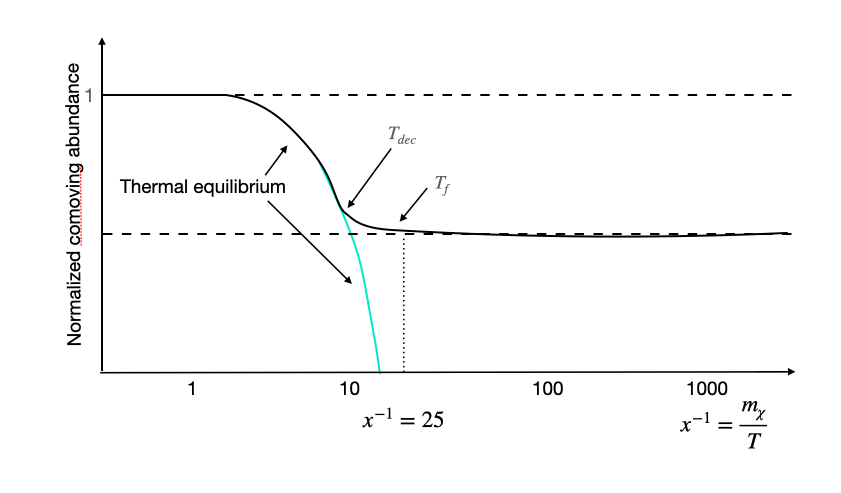
\includegraphics[width=\textwidth]{figures/schematic_thermal_eq_evolution_DM.png}
    \caption{Transition of dark matter from thermal equilibrium to freeze out. Both the decoupling temperature (where dark matter stops being in thermal equilibrium with luminous matter) and the freeze out temperature (when the rate of expansion has dropped the annihilation rate to negligible amounts, so that the comoving density can be considered constant) are indicated on the schematic. Figure is based on the figure in \cite{Baer}}
    \label{fig:DM_thremal_eq_freeze_out}
\end{figure}



\subsubsection{Other dark matter models}\label{IntroOtherDM}
WIMP dark matter is not the only dark matter model on the market, indeed, dark matter models span over $\approx$ 30 orders of magnitude in mass. A collection of models and their mass ranges is shown in figure \ref{fig:DarkMatterModelsSummary}. Notable other dark matter candidates are neutrinos, sterile neutrinos, axions and primordial black holes (not shown in figure \ref{fig:DarkMatterModelsSummary}). In this section we shall briefly discuss their main concepts, advantages and disadvantages. Promising candidates usually share the quality that they solve not just the nature of dark matter, but also another problem in physics. As discussed earlier, the WIMP neutralino was considered the supersymmetric extension to the standard model at its inception.\\

\begin{figure}[h!]
    \centering
    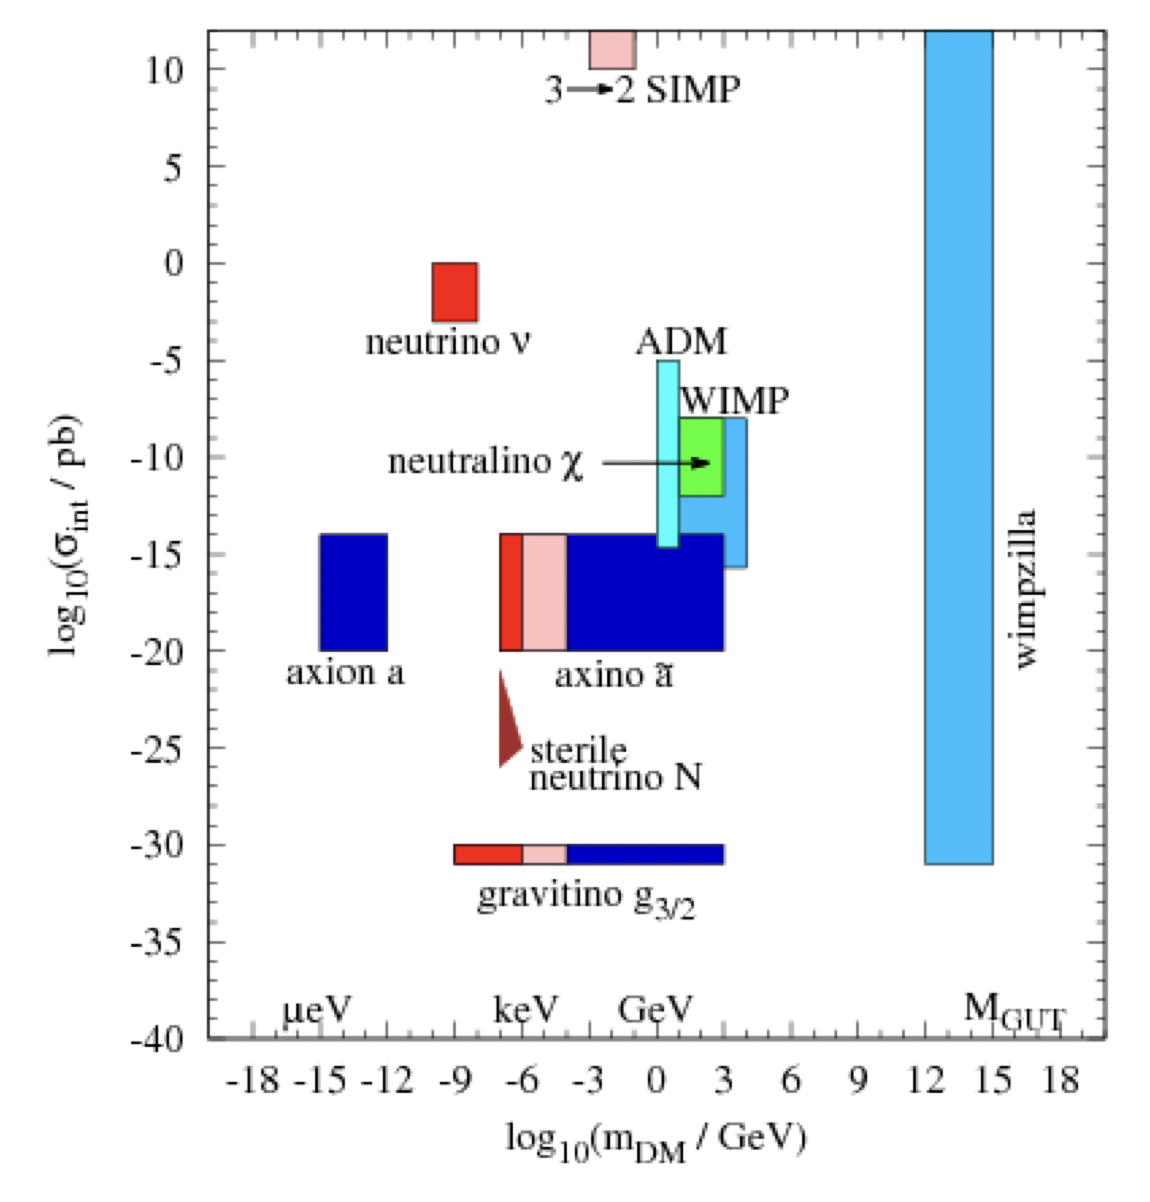
\includegraphics[width=\textwidth]{figures/DM_summary_models.png}
    \caption{Collection of candidate dark matter models over a wide mass range. The most prominent candidates are WIMP dark matter, axion dark matter and sterile neutrinos. Primordial black hole dark matter is not shown on this plot. Figure taken from \cite{BAER20151}.}
    \label{fig:DarkMatterModelsSummary}
\end{figure}



Let us first consider axion dark matter. Axions arise naturally in the Peccei-Quinn (PQ) solution to the strong CP problem\cite{PQ_axion, Weinberg} (see section \ref{sec:IntroSymmetries} for more details), by arguing that the CP violating term $\bar{\theta}$ of the QCD Lagrangian is relaxed to 0 due to an additional PQ symmetry. This symmetry is accompanied by a scalar field which spontaneously breaks the symmetry at low energy, giving rise to the axion. While the initial model, which predicted axion masses of order O(100keV) has long since been experimentally ruled out, it has been replaced by models using the same mechanism to dynamically solve the strong CP problem. Axions of such fields are expected to have masses in the $\mu$eV range. As a side effect, the scalar field would populate the universe with axions, which -- since they are produced non-thermally at rest\cite{cookbook} -- would be considered cold dark matter even though they have such low masses. As such, a dark matter theory which is not at least partially made up of axions has to provide an alternate solution to the strong CP problem. \\

Out of all the standard model particles, the neutrino is the only particle which does not interact through either the strong or electromagnetic forces. This makes it a promising initial candidate for dark matter. However, the present-day abundance of neutrinos would be given by equation \ref{eq:NeutrinoAbundance} (further details can be found in \cite{BAER20151}). Current constraints on the sum of the neutrino masses $\sum m_\nu$ limit the amount of dark matter in the form of neutrinos to about 0.5\%-1.6\% \cite{PDG2022}. These constraints come from neutrino mixing experiments, as well as from cosmological bounds. This is because neutrinos -- being hot dark matter -- have a direct impact on large scale structure formation. A related dark matter model is that of sterile neutrinos. This group of models postulates that the right handed neutrinos (and left-handed antineutrinos), are far more massive than their chiral partners. Since they interact only gravitationally (neutrinos carry no electromagnetic or color charge, and the weak force couples only to left-handed neutrinos and right-handed antineutrinos), they would constitute a viable candidate for dark matter\cite{}. Recent observations of neutrino mixing \cite{}, show that neutrinos are not massless but have a finite mass. The higgs mechanism responsible for giving SM particles their mass requires both left-handed and right-handed fermions \cite{}, and thus suggests the existence of the neutrinos' chiral partners. Their mass also means that their chirality is not relativistically invariant, since their velocities are slower than the speed of light; i.e. it is possible for an observer to travel faster than the neutrinos and thus observe them with a different chirality. However, it is not known why the couplings to for the left- and right-handed neutrinos would be so different. \\

\begin{equation}\label{eq:NeutrinoAbundance}
    \Omega_\nu h^2 = \frac{\sum m_\nu}{91.5 \mathrm{eV}}
\end{equation}

The final dark matter candidates to consider are primordial black holes. They are discussed more closely in section \ref{Res:PBH}, but a brief overview is given here for completeness. Very shortly after the big bang (O($10^{-23}$)s), overdense regions in the universe might have collapsed into black holes. Depending on the time of their formation, they would have consumed most the of available mass within their observable universe at the time, i.e. within their horizon. Such black holes would have expected masses today ranging over many orders of magnitude, well below the critical mass for a stable black hole \cite{HAWKING1974}. Black holes below this mass tend to radiate energy off at a rate faster than their mass accretion, via Hawking radiation \cite{VISSER_2003, HAWKING1974}. The rate at which such small black holes radiate off energy is higher the smaller they are, meaning towards the end of their lifetime they disappear via runaway evaporation. During such a process, new antiparticles and particles can be produced. Such primordial black holes fit the required properties of dark matter, being colissionless uncharged matter which interacts gravitationally. However, due to null observation of the particles expected to be released from the evaporation of black holes, their abundance can be tightly constrained. As such, they can at most make up a tiny fraction ($\approx 10^{-11}$) of the observed dark matter in our galaxy.

\subsubsection{Dark matter annihilations into antinuclei}
The null results from searches for direct detection of WIMPs, either from evidence for supersymmetry at the LHC or from direct detection experiments \cite{XENON2, Lux}, have motivated other probes for WIMPs. Antinuclei observations from WIMP annihilations have become one of the most promising of such probes, since many WIMP candidates are expected to produce a detectable flux of low energy antinuclei\cite{Ibarra:2012cc, Korsmeier:2017xzj}. By definition WIMPs can couple weakly to standard model particles, and their wide plausible mass range leaves open a large parameter space with sufficient energy to create antinuclei. Additionally, since dark matter is expected to be cold, the production of antinuclei occurs in the galactic rest frame, providing no boost to artificially increase their momentum. Thus, considering WIMP annihilations into an initial standard model state, the production of antinuclei is plausible. In a given point in space, the amount of antinuclei produced is then dependent on the number of dark matter annihilations times the spectrum of produced antinuclei in such annihilations, as given in equation \ref{eq:IntroDM_source_term}

\begin{equation}\label{eq:IntroDM_source_term}
    q(\vec{r}, E) = \frac{1}{2} \left( \frac{\rho_{\chi}(\vec{r})}{m_\chi}\right)^2 <\sigma v > (1+\epsilon) \frac{dN}{dE}
\end{equation}
, where $\rho_\chi$ is the measured dark matter density at a given point, and (1+$\epsilon$) accounts for the contribution from other annihilation products which later decay into the antinucleus in question. This process is discussed in more detail in section \ref{sec:AntinucleiInTheCosmos}.


\subsubsection{Majorana vs. Dirac dark matter}\label{sec:IntroMajoranaDiracDM}
To current knowledge, every fermion in the standard model has an antiparticle, with the same mass and quantum numbers, but opposite charge. This was first predicted by Paul Dirac, who realised that the wave equation he developed to account for special relativity in the motion of electrons implied a second solution, corresponding to a particle with opposite charge\cite{Dirac}. This particle, the positron, was subsequently discovered, and was the first discovery of antimatter\cite{positron_discovery}. \\

However, it is mathematically possible for a particle to be its own antiparticle; such particles are called Majorana particles. Out of the fermions in the standard model, only the neutrino could be a majorana particle, since all other fermions have known antiparticles. The majorana nature of the neutrino is being investigated by searching for neutrinoless double beta decay, a process by which two beta decays happen almost simultaneously, the produced neutrinos annihilate and thus provide additional energy to the electrons. The GERDA experiment is currently looking for such an effect \cite{GERDA}, but has so far found no signal. \\

WIMP dark matter is often assumed to be a majorana fermion. Given the lack of any known majorana particles, this seems somewhat unintuitive. The reason is mainly historical, since the original motivation for the WIMP was the supersymmetric neutralino, which is a hypothetical Majorana particle \cite{Supersymmetry_primer}. The reason this convention is still used, is that the effects of the assumption on the Dirac or Majorana nature of a WIMP are degenerate with the assumed WIMP self-annihilation cross section and therefore they produce the same signal. To show this, let us consider equation \ref{eq:IntroDM_source_term}, which describes the source term for antinuclei from Majorana dark matter annihilations. The Dirac nature of the WIMP enters the equation in two ways. First, the density considered. Since the total gravitational effect of dark matter is known, the total measured dark matter density is the sum of the densities of dark matter and anti dark matter $\rho_{\mathrm{DM}}^{\mathrm{meas}} = \rho_\chi  + \rho_{\overline{\chi}}$.Thus -- assuming symmetric populations of dark matter and anti-dark matter -- the density term in equation would be $\rho_\chi \rho_{\overline{\chi}} = \frac{\rho_{\mathrm{DM}}^2}{4}$. This is a factor of 2 lower than original density term (the symmetry factor of 1/2 in equation \ref{eq:IntroDM_source_term} is due to the Majorana nature and thus falls away). However,the second effect is on the thermally averaged annihilation cross section $<\sigma v>$. When predicting the value of $<\sigma v>$ required for the currently observed abundance (as was done in section \ref{sec:IntroWIMPs}) the same density alteration is required, which means that the prediction for the thermally averaged cross section remain the same. This is shown in figure \ref{fig:sigmaV_DiracvsMajorana}. Thus, these two effects cancel, yielding the same results for Dirac or Majorana dark matter. \\

\begin{figure}[h!]
    \centering
    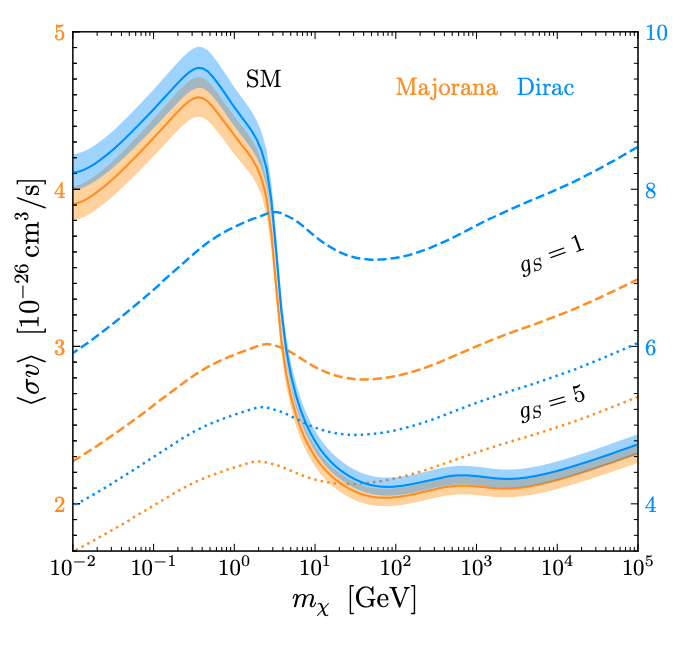
\includegraphics[width=0.7\textwidth]{figures/sigma_v_dirac_majorana_dm.png}
    \caption{Thermally averaged annihilation cross section for WIMP dark matter necessary to reproduce the measured present-day abundance of dark matter. The left y-axis shows the values for Dirac dark matter, while the right y-axis shows the values for Majorana dark matter, showing the difference of a factor 2. Taken from \cite{}. }
    \label{fig:sigmaV_DiracvsMajorana}
\end{figure}

The only possible difference between the two models would come from an asymmetry in the population of dark matter and anti dark matter, and only if this was created after decoupling. If the asymmetry was caused prior to decoupling, the derivation for the expected WIMP cross section would account for this. Thus, such an asymmetry would have had to be caused by a process after dark matter decoupled from thermal equilibrium, which suggests it would have had to form through purely dark matter interactions. It is therefore difficult to suggest any process which would cause such an asymmetry. However, assuming an asymmetry was formed, the number of annihilation would be reduced by the factor $4x(1-x)$ in respect to the case of symmetric Dirac dark matter, where $x = \rho_\chi / \rho_{\chi + \overline{\chi}}$ is the asymmetry factor. For further discussion of asymmetric dark matter, see section 4D in \cite{BAER20151}. 

%\subsubsection{The distribution of dark matter within our galaxy}
%This is carefully explained in a later section, doesnt need to be explained here i think. 
\subsubsection{The search for dark matter: the link between WIMP dark matter and antinuclei}
Searches for dark matter can be classed into 3 categories: production searches, direct detection experiments and astrophysical searches. Production searches look to detect the production of dark matter particles in high energy collisions at accelerators. Technically, if WIMP dark matter is weakly interacting and within a mass range which can be produced at accelerators, it might be detectable. However, there is currently no evidence for the production of dark matter at accelerators. Such production searches usually form only a small part of the physics programs of accelerator experiments. The second category of experiments are direct detection experiments. These experiments look for WIMP-nucleon interactions and the corresponding recoil, and include the XENON \cite{XENON_new_physics, XENON2} and LUX collaborations\cite{Lux}. These will be discussed in more detail in section \ref{sec:AntinucleiInTheCosmos}.\\

The final probes are astrophysical searches. These focus on signals produced by potential WIMP dark matter which can be differentiated from standard model sources. These signals can come either from annihilations or decay of WIMP dark matter\footnote{Technically WIMP dark matter could also scatter of baryonic matter, but this would be much easier to observe in direct detection experiments than in space.}, and we have to chose detection channels in which we could both get a reliable signal and differentiate it from other cosmic sources. The most promising searches are gamma rays and antinuclei \cite{Conrad2017}, both of which could be produced in the annihilation of many WIMP candidates, and would produce signals which are expected to be distinguishable from common astrophysical backgrounds. This thesis focuses on measuring antinuclei inelastic cross section and their effect on such an antinuclei signal, in order to help interpret any future antinuclei measurements in cosmic rays.


%\subsection{Dark matter and its connection to antinuclei}

\subsubsection{The evidence for dark matter}
\subsubsection{WIMP dark matter and the WIMP miracle}\label{sec:IntroWIMPs}
\subsubsection{Dark matter annihilations into antinuclei}
\subsubsection{Majorana vs. Dirac dark matter}\label{sec:IntroMajoranaDiracDM}
Since the properties of dark matter are not know beyond its gravitational pull, it is also not known if dark matter is its own anti-particle. 
\subsubsection{Thermal self-annihilation cross section in the early universe}
\subsubsection{The ditribution of dark matter within our galaxy}
\subsubsection{The search for dark matter: the link between WIMP dark matter and antinuclei}